\documentclass[12p, a4paper]{article}

\usepackage[headsepline, footsepline]{scrlayer-scrpage}
\usepackage[hidelinks]{hyperref}

\pagestyle{scrheadings}
\ihead{Bachelorabschlussarbeit}
\ohead{\headmark}
\automark{section}
\ifoot{Felix Bauer}
\ofoot{\pagemark}
\setlength{\tabcolsep}{10pt}
\renewcommand{\arraystretch}{1.5}

\usepackage{listings}
\lstset{numbers = left, numberstyle = \tiny, numbersep = 5pt, language = C, keywordstyle = \color{blue}, stringstyle = \color{teal}, commentstyle = \color{gray}, morecomment = [l][\color{orange}]{\#}, caption={\protect\filename@parse{\lstname}\protect\filename@base\\.\protect\filename@ext},
basicstyle=\sffamily}
\renewcommand{\lstlistingname}{Codeausschnitt}
\usepackage{pdfpages}
\usepackage[ngerman]{babel}
\usepackage[utf8]{inputenc}
\usepackage[top = 25mm, bottom = 20mm, left = 25mm, right = 25mm]{geometry}
\usepackage[onehalfspacing]{setspace}
\usepackage{graphicx}
\graphicspath{{./images/}}
\usepackage{acronym}


\begin{document}
	% !TEX root=BA-Bauer.tex

\begin{titlepage}
	\begin{center}
		\Huge
		\vspace*{2cm}
		\textbf{Entwicklung eines Aufnahme- und Wiedergabegerätes für DMX-Daten}
		
		\Large
		\vspace{2cm}
		Bachelorabschlussarbeit\\
		\vspace{.5cm}
		von\\
		\vspace{.5cm}
		Felix Bauer\\
		\vspace{1cm}
		Im Studiengang B.Eng Elektrotechnik/Informationstechnik\\ mit Schwerpunkt Mess- und Automatisierungstechnik\\
		\vspace{.5cm}
		an der HAWK Hochschule für angewandte Wissenschaft und Kunst\\ Hildesheim/Holzminden/Göttingen\\ Fakultät Ingenieurwissenschaften und Gesundheit in Göttingen\\
		\vspace{1.5cm}
		
\includegraphics[scale = 1.4]{HAWK-Logo}\\
		\vspace{1.5cm}
		Erstprüfer: Prof. Dr. rer. nat. Roman Grothausmann\\
		Zweitprüfer: Dipl.-Ing. Tobias Bürmann\\
		\vspace{.5cm}
		\today
		
		\vfill
	\end{center}
\end{titlepage}
	% !TEX root = BA-Bauer.tex

\includepdf[pages = 2]{./documents/BA Antrag Abschlussarbeit & Kolloquium Fak_I}
	% !TEX root = BA-Bauer.tex
\newpage
\noindent\begin{minipage}[c][.99\textheight][c]{\textwidth}
	\centering
	\begin{minipage}{.65\linewidth}
		%\centering
		\textbf{Gender Erklärung}\\
		\newline
		%\vspace{.5cm}
		Aus Gründen der besseren Lesbarkeit wird in dieser Bachelor-abschlussarbeit das generische Maskulin verwendet. Dabei sind weibliche und anderweitige Identitäten des Geschlechts ausdrücklich gleichermaßen gemeint.
	\end{minipage}
\end{minipage}
	% !TEX root=BA-Bauer.tex

\renewcommand*\contentsname{Inhaltsverzeichnis}
\tableofcontents
	\input{Abkürzungsverzeichnis}
	% !TEX root = BA-Bauer

\newpage
\section{Einleitung}
Einmal pro Jahr wird die Nacht der Kultur in der Göttinger Innenstadt veranstaltet, ein vielfältiges Stadtfest der Kulturszene. Das Göttinger Wahrzeichen, das Gänseliesel, soll eindrucksvoll mit bewegtem und statischem Licht in Szene gesetzt werden. Für den Lichttechniker bedeutet diese Aufgabe die Installation und Verkabelung aller Lampen, die Programmierung einer Lichtshow und die Betreuung dieser während der ganzen Nacht. Die Lichtshow wird von einem Laptop mit DMX-Interface oder von einem Lichtsteuerpult aus gesteuert. Der Diebstahl eines dieser Geräte würde einen großen finanziellen Verlust bedeuten. Mit dem Gerät, welches in dieser Arbeit entwickelt wird können die Daten der vorab programmierten Lichtshow aufgezeichnet werden. Am Tag der Veranstaltung muss der Lichttechniker nur noch die Lampen installieren, verkabeln und die gespeicherte Lichtshow von dem Gerät abspielen. Damit bleibt ihm Zeit, die Veranstaltung als Gast zu genießen.\\
Die in der vorangegangenen Praxisprojektarbeit erarbeiteten Grundlagen zur Aufnahme und Wiedergabe von DMX-Daten haben die technische Umsetzbarkeit aufgezeigt. Der entwickelte Prototyp ist in seiner Funktionalität jedoch sehr eingeschränkt und ist den Anforderungen eines realen Anwendungsfalls nicht gewachsen. Ziel dieser Arbeit ist die Weiterentwicklung und Erweiterung der erarbeiteten Inhalte, sowie die Implementierung in einen Prototypen des marktfähigen Produktes.\\
%Umstand eigener Bedarf: um ein pers Problem zu lösen, war es notwendig sich mit der Materie auseinanderzusetzen. das resultierte in großem Interesse für das Kernthema der BA
%Für die Entwicklung werden hauptsächlich Kenntnisse der Elektrotechnik, besonders aus dem Bereich der Schaltungstechnik und Informatik verwendet. 
%Motivation: pers. Interesse 
%Schaltungselektronik, Platinendesign, Informatik, CAD, 3D-Druck, 
Zu Beginn wird das Grundprinzip der benötigten elektrischen Schaltung erläutert. Daraufhin werden die für die Umsetzung des Prinzips benötigten Hardwarekomponenten und deren Beschaltung näher erläutert, sowie deren Funktion in der Gesamtschaltung aufgezeigt. Anschließend wird gezeigt, wie die abstrakte Schaltung in ein reales Platinendesign überführt wird. Die Platine wird in einem Gehäuse montiert, dessen Konstruktion und Design dargestellt wird. Nach der Behandlung der Hardware werden die wichtigsten Funktionen der Software betrachtet und in den Gesamtkontext gestellt. Dafür wird zunächst auf die grundlegende Softwarearchitektur eingegangen und die verwendeten Hilfsmittel, die zur Konfiguration der Hardware und Entwicklung der Software verwendet werden, werden vorgestellt. Die wichtigsten Funktionen, die zur Verarbeitung der Eingaben des Benutzers benötigt werden, und die Funktionsweise der Benutzer-Rückmeldungen für die einzelnen Komponenten werden erläutert. Die überarbeitete Aufnahme- und Wiedergabefunktion, sowie die neu hinzugekommenen Modi werden außerdem erläutert. Zuletzt wird auf den Aufbau und die Umsetzung des Menüs und der entsprechenden Menüführung, sowie auf die Einstellungsmöglichkeiten eingegangen.
%Paar Funktionen nennen.
	% !TEX root = BA-Bauer

\newpage
\section{Ziel der Arbeit}
\label{sec:Ziel}
In dieser Arbeit werden die in der vorangegangenen Praxisprojektarbeit erarbeiteten Funktionsprinzipien für die Aufnahme und Wiedergabe von DMX-Daten mit einem Mikrocontroller weiterentwickelt und in ein für den Endbenutzer ausgerichtetes Gerät implementiert. Ziel dabei ist die Herstellung eines Prototyps eines DMX-Aufnahme und -Wiedergabegerätes, welches eine gewisse marktreife darstellt. Zusätzlich zu den Inhalten der Praxisprojektarbeit wird eine umfassende Benutzerschnittstelle entwickelt, mit der dem Benutzer ohne spezielle Vorkenntnisse die Bedienung des Geräts ermöglicht wird. Konkret werden Taster und Drehgeber für die Eingaben des Benutzer, ein Display und LEDs für Rückmeldungen an den Benutzer verwendet. Durch die Zunahme an Funktionlität und Anzahl der Komponenten wird außerdem die elektrische Schaltung der Praxisprojektarbeit dementsprechend erweitert und an bereits vorhandenen Stellen optimiert. Für die erweiterte Schaltung wird eine Platine entwickelt, hergestellt und bestückt. Zudem wird ein passendes, kompaktes Gehäuse für die Platine gestaltet und Hergestellt. Damit ist bereits die optische Sichtweise auf eine gewisse Marktreife sichtbar.

Für die neu hinzugekommene Benutzerschnittstelle sind nicht nur die Komponenten wichtig, sondern auch die Software die sie steuert. Dafür wird entsprechender Programmcode entwickelt der dem Benutzer sinnvolle und auswertbare Rückmeldung gibt und ihm eine intuitive Bedienung des Gerätes ermöglichen. Dem Benutzer sollen außerdem Möglichkeiten gegeben sein, gewisse Einstellungen vorzunehmen um die Funktion des Gerätes auf die eigenen Bedürfnisse anzupassen. Ein besonderes Augenmerkt liegt auf der Optimierung der Aufnahme, Wiedergabe und Speicherung der DMX-Daten. Auch hier sollen dem Benutzer möglichst viele Freiheiten eingeräumt werden. Die in der Praxisprojektarbeit erarbeiteten Grundlagen werden dafür verwendet, erweitert und optimiert. Zudem werden die Optimierungsvorschläge der Praxisprojektarbeit berücksichtigt und zum Teil umgesetzt. Für die Entwicklung des Gerätes sind folgende Haupt- und Nebenanforderungen definiert.\\
\newline
\textbf{Hauptanforderungen:}\\
- Möglichkeit mehrere Aufnahmen anzulegen\\
- Einstellbare Aufnahmezeit\\
- Aufname eines DMX-Stroms und einzelner DMX-Datenpakete\\
- Benutzerschnittstelle mit Display und Menüführung\\
- Maßgeschneidertes Platinendesign\\
- Gehäuse\\
- Handliche Größe\\
\newline
\textbf{Nebenanforderungen:}\\
- Intuitive Benutzerschnittstelle\\
- Optisch Ansprechendes Design des Gehäuses\\
- Optimierung des Speicherbedarfs auf der SD-Karte\\
- Möglichkeit die Wiedergabegeschwindigkeit während der aktiven Wiedergabe zu ändern\\
	% !TEX root = BA-Bauer

\newpage
\section{Hardware}
In den folgenden Kapiteln wird auf die in dieser Arbeit verwendete Hardware eingegangen. Zunächst wird das grundlegende Pinzip der Schaltung erläutert. Daraufhin werden die Bestandteile bzw. Module im Einzelnen näher erläutert und deren Funktionsweise und Funktion in der Gesamtschaltung erklärt. Abschließend wird erläutert, wie die abstrakte Schaltung in ein Platinendesign überführt und wie diese in einem Gehäuse plaziert wird. Die Datenblätter der Hardwarekomponenten befinden sich im Anhang \ref{CD-Anhang}.
% !TEX root = BA-Bauer

\subsection{Schaltungsprinzip}

In diesem Kapitel wird auf das grundlegende Prinzip der Schlatung eingegangen. Auf die einzelnen Komponenten und deren nötige Beschaltung wird in den folgenden Kapiteln eingegangen. Generell wird bei der Entwicklung der Schaltung darauf geachtet, dass möglichst keine fertigen Modulbausteine verwendet werden. Dadurch ergibt sich in der Regel ein Preisvorteil und das industrielle Bestücken einer Platine ist einfacher.%(Quelle?)
Abbildung \ref{fig:Schaltungsrinzip} zeigt das grundlegende Prinzip der Schaltung. Auf der linken Seite steht der Benutzer des Gerätes, der das Gerät durch Eingaben bedienen kann und entsprechende Rückmeldungen erhält. Die grüne Fläche spiegelt dasGerät wieder, welches mit der DMX-Quelle, bzw. der DMX-fähigen Lichttechnik kommuniziert. Im Folgenden wird auf die Bestandteile des Gerätes eingegangen.

\vspace*{5mm}
\begin{figure}[h]
	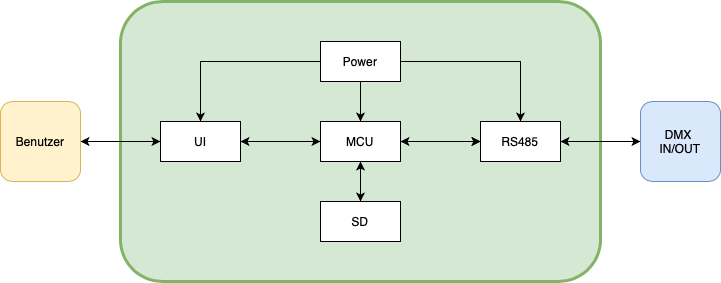
\includegraphics[width = \textwidth]{Schaltungsprinzip}
	\caption{Schaltungsprinzip}
	\label{fig:Schaltungsrinzip}
\end{figure}
\hspace*{-5mm}\textbf{Mikrocontroller (MCU)}\\
Der MCU bildet das Herzstück der Schaltung, über den sämtliche Kommunikation für die Benutzerschnittstelle, den DMX-Ein- und Ausgang und die SD-Karte läuft. Aufrgund der hohen Anforderungen an den MCU wird bei der Entwicklung ein besonderes Augenmerk auf ihn gelegt. Die Auswahl des MCUs richtet sich an dem in der vorangegangen Praxisprojektarbeit verwendeten Mikrocontroller. Auswahlkriterien sind eine mindestens gleichhohe Taktfrequenz des Prozessors, eine verfügbare UART-Schnittstelle, eine SDIO-Schnittstelle und mindestens drei Timer.\\
\textbf{Spannungsversorgung (Power)}\\
Die Spannungsversorgung für alle Komponenten wird von einer USB Schnittstelle geliefert, welche keine Daten übertragt. Über die USB-Schnittstelle werden 5V geliefert (Quelle), welche dann in enstprechend benötigte Spannungen gewandelt werden. Besonders kritisch ist die Versorgung des MCUs. Unter normalen Betriebsbedingungen darf die Versorgungsspannung nur soweit einbrechen, dass der MCU weiterhin den darauf befindlichen Programmcode fehlerfrei ausführen kann.\\
\textbf{Benutzerschnittstelle (UI)}\\
Damit der Benutzer das Gerät bedienen kann, ist ein Informationsfluss in zwei Richtungen eforderlich. Zum einen müssen Eingaben durch den Benutzer erfasst werden, zum anderen muss das Gerät dem Benutzer eine Rückmeldung ausgeben können. Für die Benutzereingaben werden Taster und ein Drehgeber (Encoder) verwendet. Durch den Einsatz von Tastern können präzise und zeitgenaue Eingaben vom Benuter vorgenommen werden, an Stellen an denen es nötig ist, zum Beispiel beim starten einer Wiedergabe. Der Encoder hingegen bietet die Möglichkeit viele Eingaben in kurzer Zeit zu tätigen, zum Beispiel wenn die Aufnahmezeit eingestellt wird.\\
\textbf{RS485}\\
Die RS485-Schnittstelle ist die Verbindung zwischen DMX-Quelle/Senke und dem MCU, welche notwendig ist, da der MCU keine RS485 konformen Signalpegel liefern kann. Zudem werden durch die Schnittstelle die DMX-Leitungen galvanisch von der restlichen Schaltung getrennt. Spannungs- und Stromspitzen ausgehend von den DMX-Leitungen können so die Schaltung nicht beeinträchtigen oder beschädigen.\\
\textbf{Speicher (SD-Karte)}\\
Damit ein sinnvoler Einsatz des Gerätes mögilch ist, ist es notwendig die aufgenommenen Daten auf einem Speichermedium zu sichern und diese nach einen Neustart des Gerätes nach wie vor verfügbar sind. In der vorangegangen Praxisprojektabreit wurde bereits gezeigt, dass der Einsatz einer SD-Karte für diesen Zweck geeignet ist. Die Verwendung einer SD-Karte ermöglicht dem Benutzer außerdem eine gewisse Sicherheit in Bezug auf den Schutz der Daten. Sollte ein Gerät einen Defekt aufweisen, so kann einfach ein neues Gerät mit der bereits beschriebenen SD-Karte bestückt werden. Zudem können für verschiedene Einsatzgbiete auch verschiede SD-Karten verwendet werden.
% !TEX root = BA-Bauer

\subsection{STMicroelectronics STM32F446ZE}
\label{sec:STM}
Aufgrund der aktuellen Corona-Pandemie und einer damit einhergehenden Siliziumchip-Knappheit kann für die Entwicklung nicht der gleiche MCU verwendet werden, wie in der Praxisarbeit. Die Eckdaten beider Mikrocontroller sind allerdings ähnlich. Abbildung \ref{fig:MCU_pinout} zeigt die Pinbelegung des Chips. Insgesamt stehen bis zu 20 Schnittstellen und 114 interruptfähige Ein- und Ausgangsports, von denen 112 5\,V-tolerant sind, zur Verfügung. Der interne 512\,kBytes große Flash-Speicher und 128\,kByte SRAM bieten genügend Kapazität für einen großen Programmcode, sowie genügend Platz für Heap und Stack. Der STM32F446ZE arbeitet mit einer maximalen Taktfrequenz von 180MHz und basiert auf einem \textit{Arm\textsuperscript{®} 32-bit Cortex\textsuperscript{®}-M4} Prozessor \cite[S. 1]{STM32F446ZE_Datasheet}.
\begin{figure}[!htb]
	\begin{center}
		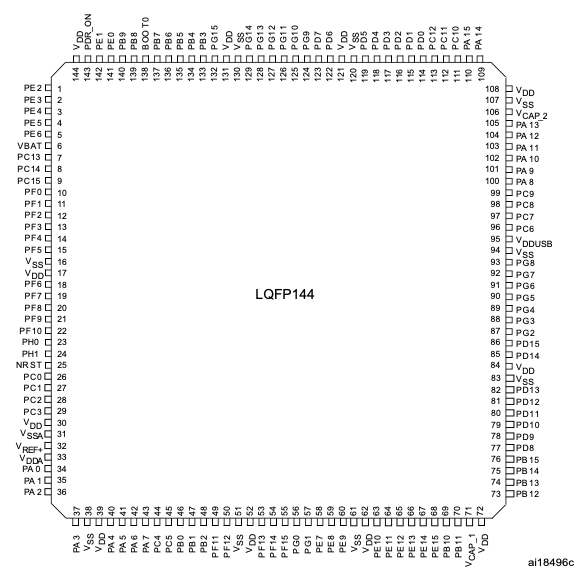
\includegraphics[scale = 0.4]{STM32F446ZE_pinout}
		\caption{STMicroelectronics STM32F446ZE Mikrocontroller Pinout \cite[S. 41]{STM32F446ZE_Datasheet}}
		\label{fig:MCU_pinout}
	\end{center}
\end{figure}\\
\newline
\hspace{-5mm}\textbf{Spannungsversorgung}\\
Die Spannungsversorgung des MCUs ist besonders kritisch, da eine einbrechende Spannung zu Fehlern bei der Ausführung des Programmcodes oder sogar zu einem kurzzeitigen Ausfall und Neustart des MCUs führen kann. Bei steigenden Schaltfrequenzen des MCUs wirken die Leiterbahnen auf der Platine induktiv, wodurch möglicherweise nicht schnell genug genügend Strom geliefert werden kann, was zu einem Einbruch der Spannung führen kann. Um dem entgegenzuwirken werden sogenannte Stützkondensatoren möglichst nah an den Versorgungsspannungs-Pins ($V\textsubscript{DD}$ und $V\textsubscript{SS}$) des MCUs platziert. Benötigt der MCU kurzzeitig einen großen Strom, so entlädt sich der Kondensator. Durch die kurze Distanz zum MCU muss der Strom über eine kürzere Strecke der Leiterbahn fließen, was eine niedrige Induktivität zur Folge hat. Aus dem Datenblatt \cite{F446RM} des MCUs kann die Dimensionierung der Stützkondensatoren entnommen werden. Insgesamt werden elf Pin-Paare, bestehend aus $V\textsubscript{DD}$ (3,3\,V) und $V\textsubscript{SS}$ (0\,V), mit 0,1\,$\mu$F Kondensatoren parallel verbunden.\\
\newline
\textbf{Taktgeber (Clock)}\\
Der MCU verfügt über einen internen Hochgeschwindigkeits-Oszillator \textit{High-Speed-Internal-Clock} (HSI) und einen Niedergeschwindigkeits-Oszillator \textit{Low-Speed-Internal-Clock} (LSI). Die HSI schwing mit einer Frequenz von 16\,MHz und ist werksseitig auf eine Abweichung der Schwingfrequenz von einem Prozent kalibriert. Um die maximale Taktfrequenz des Prozessors zu erreichen, wird eine interne Phasenregelschleife \textit{phase-locked loop}(PLL) eingesetzt. Durch die PLL kann ein Vielfaches der Oszillatorfrequenz erzeugt werden, wobei die Stabilität der Schwingung nicht eingeschränkt wird \cite[S. 270]{Ehrhardt1992}. Eine weitere Möglichkeit die Taktfrequenz zu generieren, ist die Verwendung eines externen Oszillators \textit{High-Speed-External-Clock} (HSE). Der in dieser Arbeit verwendete externe Quartz schwingt mit einer Frequenz von 25\,MHz und hat dabei eine Genauigkeit von 30\,ppm. Das entspricht einer maximalen Abweichung von ca. \(30*10^{-6}\)\,\%, also einer deutlich geringeren Abweichung im Vergleich zum internen Oszillator. Da für die Aufnahme und Wiedergabe der DMX-Daten möglichst genaue Zeitabstände benötigt werden, wird der externe Quartz verwendet.
\begin{figure}[!h]
	\begin{center}
			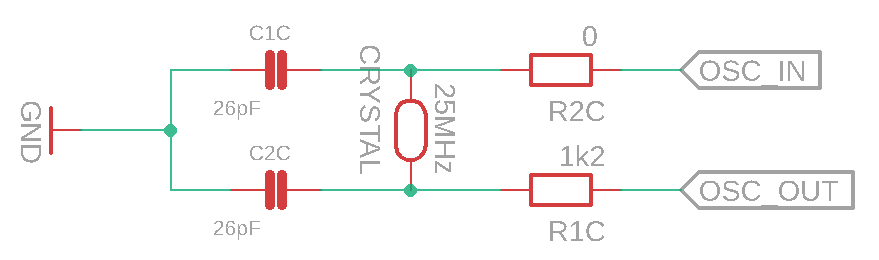
\includegraphics[scale=1]{Schaltung-Quartz}
			\caption{Beschaltung Quartz}
			\label{fig:Quartz}
	\end{center}
\end{figure}\\
Abbildung \ref{fig:Quartz} zeigt die Beschaltung des externen Quartzes. Er wird parallel zu dem Eingang $OSC\_IN$ und dem Ausgang $OSC\_OUT$ des MCUs geschaltet. Zwischen dem Ein- und Ausgang des MCUs befindet sich ein integriertes \textit{Nicht-Gatter} (Inverter) \cite[S. 11]{OscillatorAN}, welches bei einem Schaltvorgang hohe Ströme ausgeben kann. Damit kein Schaden an Quartz und MCU entsteht, wird der maximal fließende Strom durch den Widerstand \textit{R1C} am $OSC\_OUT$-Pin begrenzt. Aus Symmetriegründen befindet sich ein 0\,$\Omega$-Widerstand am $OSC\_IN$-Pin, der dafür sorgt, dass auf beiden Seiten des Quartzes die gleichen Übergangskapazitäten der Lötstellen vorhanden sind. Der Quartz wird mithilfe von zwei Lastkapazitäten mit dem 0\,V Potential verbunden. Der Wert der Kapazitäten \textit{$C_{L1}$} und \textit{$C_{L2}$} lässt sich mit folgender Formel berechnen.
\begin{equation}
		C_L = \frac{C_{L1} * C_{L2}} {C_{L1} + C_{L2}} + C_s \cite[S. 12]{OscillatorAN}
\end{equation}
\textit{$C_L$} wird vom Hersteller des Quartzes vorgegeben und beträgt in diesem Fall 18\,pF. \textit{$C_S$} ist die Kapazität der Lötstellen und Leiterbahnen zwischen dem Quartz und dem MCU, welche mit 5\,pF angenommen wird. Um möglichst wenig verschiedene Bauteile verwenden zu müssen, erhalten in der Regel die Kapazitäten $C_{L1}$ und $C_{L2}$ die gleiche Wertigkeit, wodurch die Formel wie folgt vereinfacht werden kann.
\begin{equation}
	C_{L1} =  C_{L2} = 2(C_L - C_S)
\end{equation}
Laut der Formel müssen $C_{L1}$ und $C_{L2}$ eine Kapazität von 26\,pF aufweisen. Da Kondensatoren mit dieser Kapazität nur schwer erhältlich sind wird eine marktüblichere Kapazität von 27\,pF verwendet.\\
\newline
\textbf{Serial Wire Debug-Schnittstelle}\\
Im Auslieferungszustand des MCUs befindet sich keine Software auf diesem. Mit einem Entwicklungsboard, wie es in der Praxisarbeit verwendet wurde, kann eine Software einfach über eine USB-Schnittstelle auf den MCU übertragen werden, da auf dem Entwicklungsboard ein sogenannter $programmer$ verbaut ist. Das in der Praxisarbeit verwendete Entwicklungsboard bietet die Möglichkeit, einen Teil der Platine abzutrennen und als eigenständigen $programmer$ zu verwenden, mit dem die Software mithilfe der \textit{Serial Wire Debug}-Schnittstelle (SWD-Schnittstelle) auf den MCU übertragen werden kann. Die SWD-Schnittstelle ermöglicht das Übertragen der Software und das Debuggen\footnote{Analyse und Fehlerbehebung von Programmcode} des Codes während der Laufzeit. Für die Datenübertragung zwischen MCU und PC werden nur zwei Verbindungen. Über die Leitung \textit{serial wire data}-Leitung werden die Daten gesendet, wohingegen die Leitung \textit{serial wire clock}-Leitung den Takt des Datenstroms angibt. Soll ein neues Programm auf den MCU übertragen werden, so muss er zunächst in einen speziellen Modus versetzt werden, um den Programmspeicher beschreiben zu können. Dazu muss der MCU neugestartet werden und beim Start des MCU am $BOOT0$-Pin ein High-Pegel anliegen. Sobald die Übertragung beendet ist, muss der MCU ein weiteres Mal neugestartet werden, um den Programmcode auszuführen, jedoch muss beim Start nun ein Low-Pegel am $BOOT0$-Pin anliegen. Das Anlegen der entsprechenden Pegel am $BOOT0$-Pin sowie der Neustart können per Hand durchgeführt werden, allerdings kann diese Aufgabe auch vom $programmer$ übernommen werden. Dafür müssen zwei weitere Verbindungen für den $BOOT0$-Pin und $NRST$-Pin vorhanden sein. Zuletzt ist außerdem eine Verbindung der 0\,V-Potentiale notwendig, da es sich bei allen Signalen um spannungsbezogene Signale handelt. Optional kann der MCU mit einer weiteren Verbindung vom $programmer$ mit 3,3\,V Spannung versorgt werden.\\
\newline
\textbf{NRST- und BOOT0-Pin}\\
Unter den 144 Pins des MCUs befinden sich unter anderem, wie bereits im vorigen Abschnitt erwähnt, der $NRST$- und $BOOT0$-Pin. Beide Pins sind mit externen Tastern beschaltet, um Fehler bei den Verbindungen zwischen MCU und $programmer$ zu kompensieren. Außerdem kann das Programm mit dem Betätigen eines Tasters neugestartet werden, was bei der Programmierung von Vorteil ist. Für den verkaufsfertigen Zustand des Gerätes werden die Taster allerdings nicht benötigt und können einfach weggelassen werden. 
% !TEX root = BA-Bauer
\newpage
\subsection{Maxim Integrated MAX14945EWE+ RS485 Treiberchip}

Für das Senden und Empfangen von DMX-Daten wird eine galvanisch getrennte RS485-Schnittstelle benötigt \cite[S.6-8]{Bauer2021}. Der Einsatz von einzelnen Optokopplern und einem RS-485-Treiberchip, wie in der vorangegangenen Praxisarbeit, benötigt viel Platz auf der Platine und bietet ein hohes Fehlerpotential, da ingesamt vier ICs\footnote{enlg. $integrated\ circuit$: Integrierter Schaltkreis} auf die Platine aufgebracht werden müssen. Potentielle Feherquellen sind eine hohe Anzahl an Lötstellen der ICs und dessen Beschaltung, sowie die Leiterbahnen zwischen den einzelnen Komponenten. Jedes Stück Leiterbahn kann Störungen in den Rest der Schaltung streuen, was zu Fehlern in kritischen Teilen der Schaltung führen kann, beispielsweise der SD-Karte. Die Lösung dieses Problems ist der intern galvanisch getrennte Treiberchip \textit{MAX14945EWE+} der Firma \textit{Maxim Integrated}.
\begin{figure}[h]
	\begin{center}
		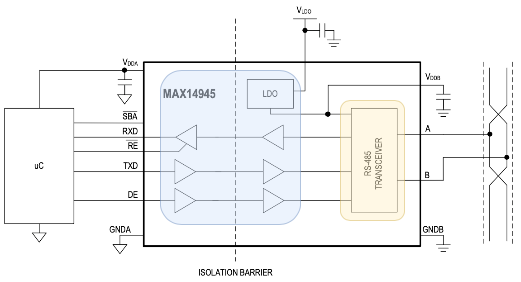
\includegraphics[width=.7\linewidth]{MAX_typical_mark}
		\caption{MAX14945EWE+ Typical Application Circuit \cite[s.19]{MAX14945MN}}
		\label{fig:MAXfd}
	\end{center}
\end{figure}
Abbildung \ref{fig:MAXfd} zeigt den schematischen Aufbau des Treiberchips inklusive dessen typischer Beschaltung. Im blau markierten Bereich befindet sich die galvanische Trennung des Chips. Die gestrichelte Linie in der Mitte markiert die Trennung der Seiten $A$ und $B$. Die Funktionen der Pins können Tabelle \ref{tab:MAX_pins} entnommen werden. Die linke Seite ($A$ Seite) ist dem Mikrocontroller zugewendet und wird mit dem 5\,V Potential der USB-Schnittstelle versorgt und mit einem 0,1\,$\mu$F und 1\,$\mu$F Kondensator in Parallelschaltung gestützt. Die Kondensatoren sollen laut Datenblatt möglicht nah am Treiberchip platziert werden. Pin $TXD$ wird mit dem Ausgang, Pin $RXD$ mit dem Eingang der UART-Schnittstelle des MCUs verbunden. Zum aktivieren des Senders oder Empfängers des Treibers muss ein entsprechender Logikpegel an den Pins $DE$ und $\overline{RE}$ anliegen. Da die Logik des Pins zum aktivieren und deaktivieren des Empfängers invertiert ist, können beide Pins kurzgeschlossen werden und mit einem Ausgang des MCUs verbunden werden. Ein interner pulldown-Widerstand an beiden Pins ermöglicht die direkte Verbindung zum MCU ohne weitere Beschaltung. Die rechte Seite ($B$ Seite) des Treiberchips muss, um die galvanische Trennung zu gewährleisten, mit einer entsprechend getrennten Spannungsquelle versorgt werden. Diese wird mithilfe eines DC/DC Konverters, der die von der USB-Schnittstelle eingehenden 5\,V isoliert und am Ausgang wieder ausgibt \cite{DC_MN}. Um eine möglichst stabile Spannungsversorgung zu gewährleisten, wird der im Treiberchip interne $low-dropout$-Spannungsregler vewendet, wodurch Pin $V_{DDB}$ als Ausgang der stabilisierten Spannung fundiert. Pin $V_{DDB}$ und $V_{LDO}$ werden mit jeweils einem 0,1\,$\mu$F und parallegeschlaltetem 1\,$\mu$F Kondensator mit $GNDB$ verbunden.
\begin{table}[h]
	\begin{center}
			\caption{Pinbeschreibung MAX14945EWE+ \cite[S.12-13]{MAX14945MN}}
		\begin{tabular}{l | l}
			\textbf{Pin} & \textbf{Funktion}\\
			\hline
			$TXD$ & serieller Dateneingang\\
			$RXD$ & serieller Datenausgang\\
			$DE$ & 1: Sender aktivieren, 0: Sender deaktivieren\\
			$\overline{RE}$ & 1: Empfänger deaktivieren, 0: Empfänger aktivieren\\
			$\overline{SBA}$ & 1: $B$ Seite inaktiv, 0: $B$ Seite funktionsfähig\\
			$A$ \& $B$ & symmetrischer Treiberausgang\\
			$V_{DDA}$ \& $GNDA$ & Spannungsversorgung $A$ Seite\\
			$V_{DDB}$ \& $GNDB$ & Spannungsversorgung $B$ Seite\\
			$V_{LDO}$ & Spannungsregler Eingang $B$ Seite
		\end{tabular}
	\label{tab:MAX_pins}
	\end{center}
\end{table}
%Abbildung \ref{fig:MAXfd} zeigt den schematischen Aufbau des Treiberchips. Die gestrichelte Linie zeigt die galvanische Trennung im inneren des ICs. Auf der linken Seite ($A$ Seite) befindet sich der serielle Eingang ($TXD$) und Ausgang ($RXD$) sowie die Pins $DE$ zum aktivieren und $\overline{$$RE$} deaktivieren des Treibers. Der invertierte Ausgang $\overline{SBA}$ gibt einen low-Pegel aus wenn die rechte Seite (B-Seite) des ICs mit Spannung versorgt ist und funktioniert. Der eigentliche Treiber, sowie dessen symmetrischer Ein- und Ausgang ($A$ und $B$) befinden sich auf Seite $B$. Außerdem finden sich insgesamt 5\,Pins für die Spannungsversorgung des ICs. Um eine vollständige galvanisch entkopplung zu garantieren muss die Spannungsversorgung der $A$ und $B$ Seite auch galvanisch entkoppelt sein. Aus diesem Grund gibt es zwei Pin-Paare, bestehend aus $VDD$ \& $GND$, für Seite $A$ und $B$. Zusätzlich steht auf Seite $B$ ein interner \textit{low-dropout} Spannungsregler (LDO\footnote{Hochempfindliche Schaltung zur linearen Regelung einer spezifischen Spannung. \cite{LDO}}) zur Versorgung der Seite $B$ zur Verfügung. Die galvanisch entkoppelte Spannungsversorgung wird mithilfe eines DC/DC-Konverters mit 5\,V Ein- und Ausgang erreicht. Gespeist wird der Konverter direkt von der USB-Buchse. Seite $B$ benötigt eine Versorgungsspannung zwischen 4,68\,V und 14\,V zwischen Pin $VLDO$ und $GNDB$, Seite $A$ eine Spannung zwischen 1,71\,V und 5,5\,V zwischen Pin $VDDA$ und $GNDA$ \cite[s. 2]{MAX14945MN}. Um Stromspitzen und den damit einhergehenden mögichen Spannungseinbruch aufzufangen werden jeweils zwei Stützkondensatoren mit einer Kapaität von 100\,nF und 1\,$\mu$F zwischen den Versorgungspins geschaltet. 
%-Preistechnis kein Nachteil gegenüber einzelnem Treiber und Optokopplern\\
%-Galvanisch getrennte Spannungsversorgung nach wie vor notwendig\\
% !TEX root = BA-Bauer

\subsection{Encoder}
\label{sec:Encoder}
Für die Benutzereingaben sind Taster und vor allem ein Encoder wichtig. Taster ermöglichen eine zeitlich präzise ein Eingabe, wohingegen ein Encoder viele Eingaben in kurzer Zeit ermöglicht. Möchte ein Benutzer eine Aufnahmezeit von 55 Sekunden einstellen, so müsste er 55 mal einen Taster betätigen, mit einem Encoder reichen wenige Umdrehungen dafür aus. In diesem Kapitel wird auf das Funktionsprinzip und die Beschaltung des vewendeten Encoders eingegangen.\\
%Formulierung: Raster bei den Umdrehung ->24
Ein Encoder besteht im einfachsten Sinne aus zwei Schaltern, wie Abbildung \ref{fig:Encoder-Schaltung} zeigt. 
\begin{figure}[h]
	\begin{center}
		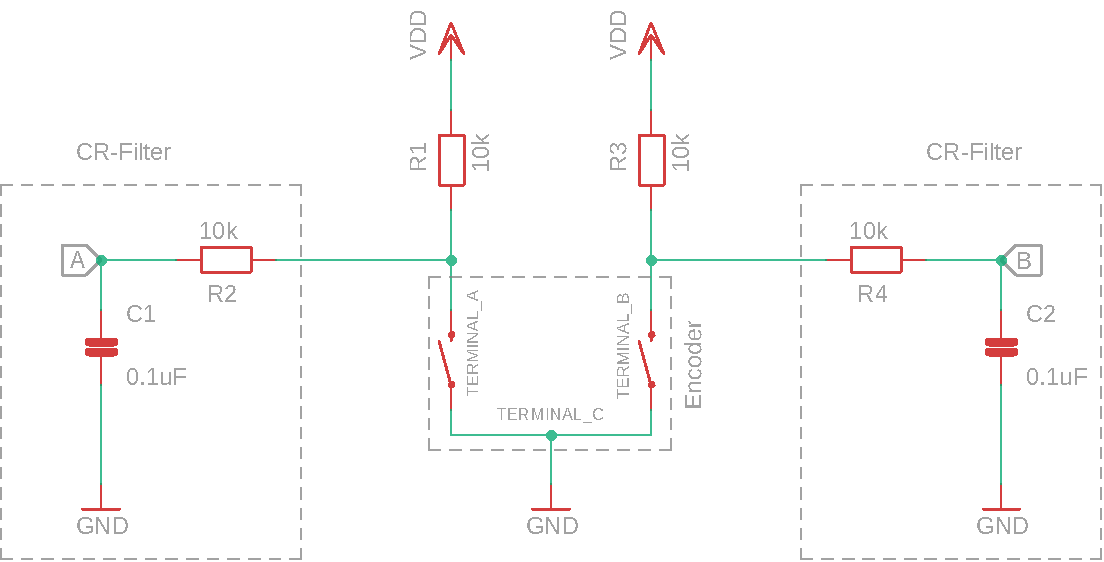
\includegraphics[angle = 0, scale = 1.2]{Encoder-Schaltung-Eagle}
		\caption{Encoder Schaltung \cite{EncoderMN}}
		\label{fig:Encoder-Schaltung}
	\end{center}
\end{figure}
Die Schalter sind auf der einen Seite intern miteinander verbunden (\textit{Terminal C}) und werden auf das 0\,V Potential geschaltet. Die andere Seite der Schalter wird direkt über \textit{Terminal A} und \textit{Terminal B} nach außen geführt. Jeweils ein exerner 10\,k$\Omega$ Pull-Up-Widerstand (R1 und R3) zieht die Ausgänge auf die Betriebsspannug von 5\,V. Ist der Schalter geöffnet, so fließt kein Strom und folglich fällt keine Spannung am Pull-Up-Widerstand ab. Am entsprechenden Terminal können 5\,V gegenüber der Masse gemessen werden. Ist der Schalter geschlossen so fällt die gesamte Spannung am Widerstand ab und am entsprechenden Terminal liegt nun Masse-Potential an. Der Hersteller des Encoders empfiehlt das Beschalten des Encoders mit zwei CR-Tiefpassfiltern um hochfrequente Schaltvorgänge zu filtern. Bei einem Schaltvorgang können die Kontakte des Schalters mechanisch schwingen und dadurch mehrfach hintereinander öffnen und schließen \cite[s. 67]{TechInfo}, wodurch mehfrache Eingaben getätigt werden, obwohl der Encoder nur um einen Schritt gedreht wurde. Die Signale des Encoder werden an Punkt A und B in Abbildung \ref{fig:Encoder-Schaltung} entnommen und über zwei Leiterbahnen zum MCU geführt. %\textbf{Mehr Erklärung??}
\begin{figure}[h]
	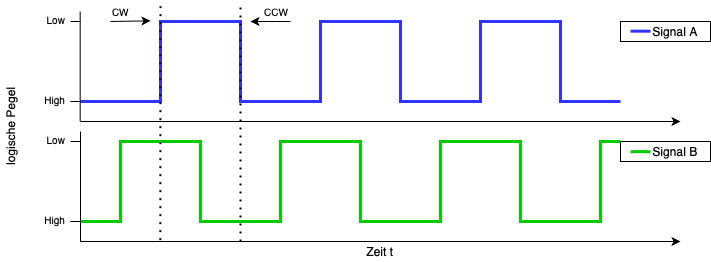
\includegraphics[width=\linewidth]{Encoder-signal}
	\caption{Encoder-Signal bei Drehung im Uhrzeigersinn}
	\label{fig:Encoder-signal}
\end{figure}
Wenn der Encoder gedreht wird schließen und öffnen die internen Schalter versetzt zueinander. Abbildung \ref{fig:Encoder-signal} zeigt die ausgehenden Signale an \textit{Terminal A} und \textit{Terminal B} im zeitlichen Verlauf bei einer gleichmäßigen Rotationsgeschwindigkeit. Durch den versetzten Rhythmus der beiden Schalter kann die Drehrichtung bestimmt werden, indem eines der beiden Signale betrachtet wird, in diesem Beispiel das Signal des \textit{Terminal A}. Ändert sich der Zustand des Signals von \textit{high} auf \textit{low} kann zunächst bestimmt weden, dass eine Drehbewegung stattgefunen hat. Ist nun der Pegel des anderen Signals \textit{high}, so handelt es sich um eine gegen den Uhrzeigersinn drehende Bewegung. Ist das Signal \textit{low}, so handelt es sich um eine mit dem Uhrzeigersinn drehende Bewegung. Die einzelnen Schritte der Schalter können haptisch vom Benutzer wahrgenommen werden. Jeweils an den Stellen an denen sich die Pegel beider $Terminals$ im high-Zustand befinden rastet der Drehregler leicht ein. Dadurch wird sichergestellt, dass sich die Signale des Encoders während der Nichtbenutzung in einem stabilen Zustand befinden. Zudem ergibt sich daraus eine zusätzliche Rückmeldung an den Benutzer während der Eingabe.\\
%-Bewusst gegen Druckknopf entschieden, da zweiter Bestätigungsknopf zur Verwirrung des Benutzers führen kann\\
% !TEX root = BA-Bauer

\subsection{Liquid Crystal Display (LCD)}
\label{sec:HardLCD}
Das Display ist das Herzstück der Benutzerschnittstelle und dadurch ein sehr wichtiger Bestandteil des Gerätes generell. Auf ihm können wichtige Informationen über den aktuellen Status des Geräts angezeigt werden und eine Menüführung in Verbindung mit den Tastern und dem Encoder gibt dem Benutzer die Möglichkeit alle Funktionen intuitiv zu bedienen. Bei der Auswahl des Display ist vor allem die Geschwindigkeit der Datenübertragung zum Display wichtig, da das Beschreiben des Displays auf keinen Fall die Aufnahme oder Wiedergabe der DMX-Daten stören darf. Aus diesem Grund wird ein einfaches Liquid-Crystal-Display (LCD) für die Anzeige von Zeichen verwendet. Insgesamt stehen 80\,Punkt-Matrizen, angeordnet in 20\,Spalten und 4\,Zeilen, zur Anzeige von Zeichen zu Verfügung, wobei jede Matrize aus 40\,Punkten (5\,Spalten x 8\,Zeilen) besteht. Die Zeichen werden in weiß auf blauem Hintergund dargestellt. Eine LED-Hintergrundbeleuchtung sorgt dafür, dass die angezeigten Inhalte auch in dunklen Umgebungen einfach abgelesen werden können.
\begin{figure}[h]
	\begin{minipage}{.45\linewidth}
		\centering
		\includegraphics[height=.15\textheight]{LCD-Vorderseite}
		\caption{LCD-Modul Vorderseite}
		\label{fig:LCD-front}
	\end{minipage}
	\hfill
	\begin{minipage}{.45\linewidth}
		\centering
		\includegraphics[height=.15\textheight]{LCD-Rückseite}
		\caption{LCD-Modul Rückseite}
		\label{fig:LCD-back}
	\end{minipage}
\end{figure}
%Literatur: serielle und paralle Datenübertragung
Im Auslieferungszustand (Abbildung \ref{fig:LCD-front} und \ref{fig:LCD-back}) besteht das Modul aus einer großen grünen Platine mit dem fest verbauten LCD darauf und einem an die 16\,Pins gelöteten $I^2C$\footnote{Bussystem zur seriellen Übertragung von Daten \cite[s.61]{MCU_in_Practice}}-Modul (kleine schwarze Platine) mit der das Beschreiben des Displays mittels serieller Übertragung möglich ist. Der Vorteil der seriellen Datenübertragung mittels $I^2C$ ist, dass nur eine Datenleitung, eine Taktleitung und das 0\,V-Potential mit dem MCU verbunden werden müssen. Ein Nachteil stellt die Übertragungsgeschwindigkeit dar, denn alle Bits müssen einzeln nacheinander übertragen werden. Geht man davon aus, dass die gleiche Taktrate bei einer parallelen Datenübertragung mit 8\,Bits erreicht wird, so ist die Übertragungsrate der seriellen Übertragen mindestens um den Faktor 8 kleiner, da zu den 8 zu übertragenden Bits eine Start-Bedingung des $I^2C$-Protokolls hinzukommt \cite[s. 62]{MCU_in_Practice}. Da die Geschwindigkeit der Übertragung von besonderer Bedeutung ist, wird das $I^2C$-Modul von dem Modul entfernt und eine parallele Datenübertragung gewählt. Insgesamt werden elf Leiterbahnen vom LCD-Modul direkt zum MCU geführt. Die einzelnen Funktionen der Pins des LCD-Moduls können Tabelle \ref{tab:LCD_Pins} entnommen werden. Die Pin-Paare $VDD$/$VSS$ und $A$/$K$ werden jeweils mit dem 5\,V und 0\,V Potential der USB-Schnittstelle beschaltet. Pin $R/\overline{W}$ wird außerdem mit dem 0\,V Potential verbunden, da das LCD-Display ausschließlich vom MCU beschrieben und nich gelesen werden soll. Die übrigen Pins werden direkt mit dem MCU verbunden. Der Kontrast des Display wird mit einer analogen Spannung an Pin $VO$ eingestellt, welche als Pulsweitenmoduliertes Signal vom MCU ausgeht.
\begin{table}[h]
	\begin{center}
		\begin{tabular}{l | l}
			\textbf{Pin} & \textbf{Funktion}\\
			\hline
			VDD \& VSS & generelle Spannungsversorgung\\
			A \& K & Anode und Kathode der LED-Hintergundbeleuchtung\\
			D0-D7 & Datenbus\\
			RS & H: Display Data, L: Display Instruction\\
			E & Enable\\
			R/W & Read/Write-Modus\\
			VO & LCD-Kontrast\\
		\end{tabular}
	\caption{LCD-Pinbelegung \cite[s. 7]{LCD_MN}}
	\label{tab:LCD_Pins}
	\end{center}
\end{table}\\
%Auf den Aufbau inklusve Treiberchips eingehen? Ist die Frage ob das für die Funktion an sich überhaupt wichtig ist.
%\textbf{Aufbau des Moduls}\\
%Die Steuerung des Displays wird durch einem im Modul vebauten $SPLC780D$-Treiberchip und zwei $SPLC063$-Treiberchips realisiert.
%\hspace*{5mm}-HDxxx Chip\\
%\hspace*{10mm}-8-Bit / 4-Bit Modus\\
%\hspace*{10mm}-Adressplätze für (Position des Cursors?)\\
%\hspace*{10mm}-Schieberegister\\
%\hspace*{10mm}-Befehl geben\\
%\hspace*{10mm}-ASCII\\
%\hspace*{5mm}-Character Darstellung\\
% !TEX root = BA-Bauer.tex

\subsection{LED}

Licht emmittierende Dioden (LED) sind ein essentieller Bestandteil der Benutzerschnittstelle für die Lokaisierung von Fehlern und der Überwachung während einer Aufnahme- oder Wiedergabe aus kurzer und großer Distanz. Insgesamt werden fünf LEDs in vier verschiedenen Farben (blau, orange, grün und rot) verbaut um dem Benutzer eine Unterscheidung auch auf große Distanz zum Gerät möglichst einfach zu machen. Ziel ist eine möglichst hardwarenahe Rückmeldung an den Benutzer zu geben. Tabelle \ref{table:LED} fasst die Funktionen der einzelnen LEDs zusammen. 
\begin{table}[h]
	\begin{center}
		\begin{tabular}{l | l}
				\textbf{LED-Farbe} & \textbf{Funktion}\\
				\hline
				blau & Eingeschaltet bei aktiver Spannungsversorgung des Geräts\\
				rot & Zustandsänderung bei eingehendem DMX-Datenpaket\\
				blau & Zustandsänderung bei ausgehendem DMX-Datenpaket\\
				orange & Eingeschaltet bei SD-Aktivität\\
				grün & Allgemeine Zustandsanzeige
		\end{tabular}
		\caption{LED Funktionen}
		\label{table:LED}
	\end{center}
\end{table}
Die erste blaue LED wird direkt an die 5\,V Versorgungsspannung, ausgehend von der USB-Buchse, über einen Widerstand zur Strombegrenzung, angeschlossen. Dadurch kann sehr einfach festgestellt werden ob das Gerät mit Spannung versorgt wird, unabhängig von der Funktion der restlichen Schaltung. Die zweite blaue und die rote LED müssen zwangsläufig per Software geschaltet werden, da der XLR Ein- und Ausgang parallel verbunden sind. Eine Unterscheidung von ein- bzw. ausgehenden Datenpaket ist so nicht möglich. Zudem haben Tests gezeigt, dass das direkte Verbinden einer LED mit einer Datenleitung die LED nur kaum bis nicht sichtbar zum leuchten bringt. Gleiches gilt für die orange LED. In einer Weiterentwicklung des Gerätes kann z.B. mithilfe einer monostabilen Kippstufe, wie einem NE555 IC \cite{NE555}, welche den eingeschalteten Zustand einer LED verlängern kann, eine hardwarenähere Lösung realisiert werden.
\begin{figure}[h]
	\begin{center}
		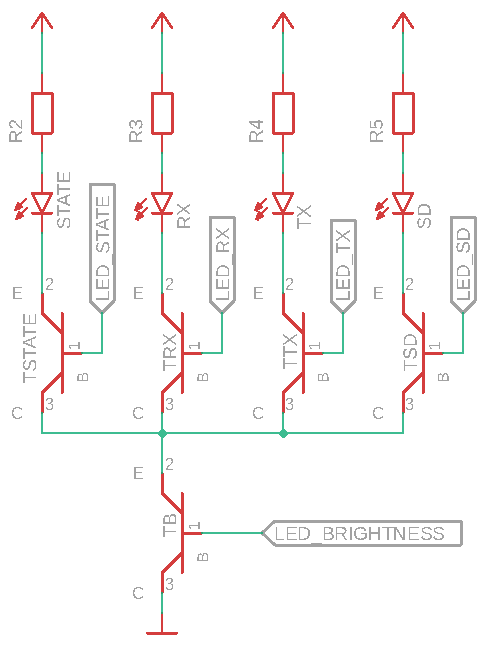
\includegraphics[scale = 0.9]{led-Schaltung}
		\caption{LED Schaltung}
		\label{fig:LED-Schaltung}
	\end{center}
\end{figure}
Abbildung \ref{fig:LED-Schaltung} zeigt die Verschaltung der von dem MCU gesteuerten LEDs. Jede LED wird mit 5\,V Spannung versorgt. Jeweils ein Widerstand begrenzt den Strom um das Durchbrennen der LED zu verhindern. Da für die vorhandenen LEDs keine Datenblätter verfügbar sind, werden alle Vorwiderstände mit 120\,Ohm dimensioniert. Das eigentliche Ein- und Ausschalten wird über jeweils einen Transistor realisiert. Die Basen des Transistoren werden mit jeweils einem Ausgang des MCUs verbunden. Der Benutzer soll die Möglichkeit besitzen die Helligkeit der LEDs je nach Anforderung zu verändern. Dazu werden die Kollektoren aller LED-Schalttransistoren auf den Emitter eines weiteren Transistors \textit{TB} geschaltet. Die Basis wird mit einem Ausgangaspin des MCUs verbunden, der mittels eines Timers ein Pulsweitenmoduliertes-Signal (PWM-Signal) ausgeben kann. Mihilfe einer Anpassung der Pulsweite kann so die Helligkeit aller LEDs reguliert werden. \\
%Hier noch mehr zu PWM schreiben. Verweis aus Kapitel Software/Einstellungen
%Dimensionierung der Vorwiderstände
%In der aktuellen Version des Aufnahmegerätes sind die Vorwiderstände aller LEDs pauschal mit 120\,Ohm dimensioniert, was in stark unterschiedlichen Helligkeiten der einzelnen LEDs resultiert. 
%\begin{figure}[h]
%	\begin{center}	
%		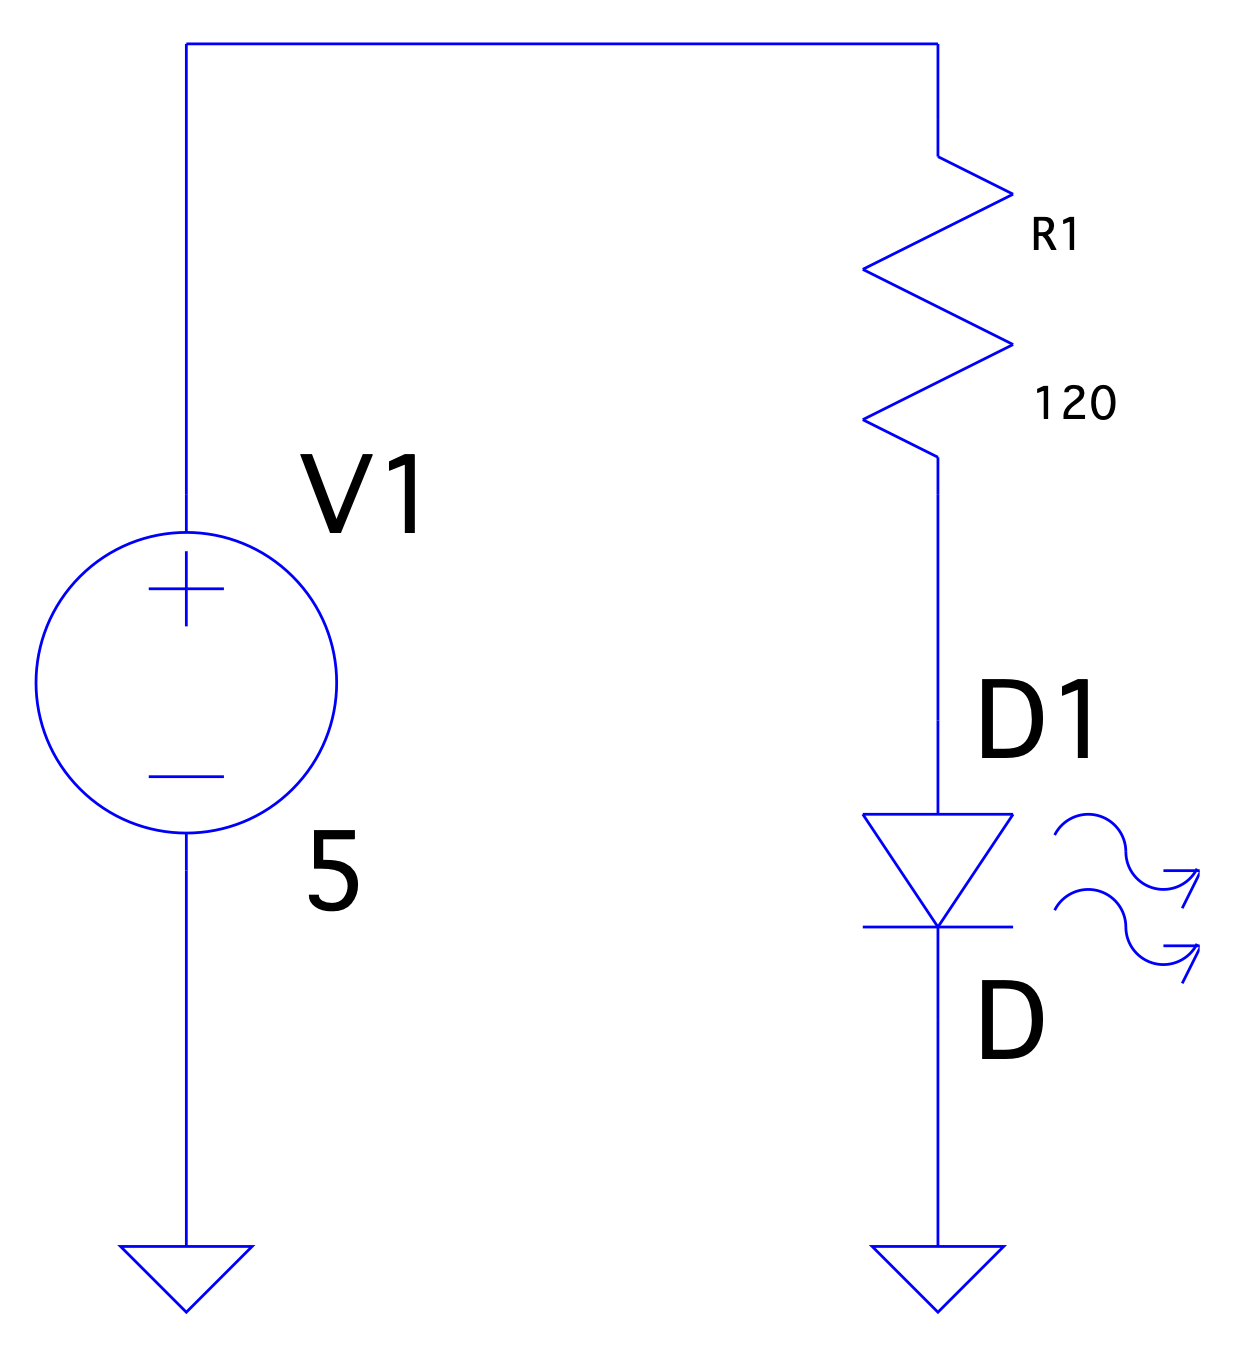
\includegraphics[width=\linewidth/4]{LED-Messung}
%		\caption{LED-Spannungsabfall Messung}
%	\end{center}
%\end{figure}
%
%\begin{table}[h]
%	\begin{center}
%		\begin{tabular}{l | l | l | l}
%			\textbf{LED-Farbe} & \textbf{$U_{LED}$} & $U_R$ & $I_{LED}$\\
%			\hline
%			blau & 3,9\,V & 0,7\,V & 5,83\,mA\\
%			rot & 2,0\,V & 2,6\,V & 21,66\,mA\\
%			grün & 2,5\,V & 1,9\,V & 15,83\,mA\\
%			orange & 2,2\,V & 2,4\,V & 20,00\,mA\\
%		\end{tabular}
%	\caption{Messung mit 120\,Ohm Vorwiderstand}
%	\end{center}
%\end{table}
% !TEX root = BA-Bauer.tex

\subsection{Spannungsversorgung}
Für eine funktionsfähige Schaltung wird eine stabile und zuverlässige Spannungsversorgung benötigt. Um die größtmögliche Kompatibilität für den Benutzer zu gewährleisten, wird das Gerät über eine USB-Schnittstelle mit der nötigen Spannung versorgt. Dadurch kann das Gerät von mobilen Akkus oder USB-Netzteilen betrieben werden. Die nachstehende Tabelle zeigt den benötigten Versorgungsspannungs- und den Strombedarf der einzelnen Komponenten. 
\begin{table}[h]
	\begin{center}
		\caption{Spannungs- und Strombedarf}
		\begin{tabular}{l | c | r }
			\textbf{Bauteil} & \textbf{Versorgungsspannung} & \textbf{Strombedarf}\\
			\hline
			MCU & 1,7\,V - 3,6\,V & max. 240\,mA\\
			RS485 Treiberchip VDDA & 1,71\,V - 5,5\,V & max. 6,6\,mA\\
			RS485 Treiberchip VDDB & 4,5\,V - 5,5\,V (isoliert)& max. 12,5\,mA\\
			DC/DC Konverter & 4,5\,V - 5,5\,V & 28\,mA\\
			LCD-Modul & 3\,V - 10\,V & 100\,mA\\
			LED & 5\,V & ca. 20\,mA\\
			SD-Kartensteckplatz & 3,3\,V & -\\
			Encoder & 5\,V & -\\
			Taster & - & -\\
			\hline
			\textbf{Gesamt} & - & max. ca. 481\,mA
		\end{tabular}
	\label{tab:VDD+IDD}
	\end{center}
\end{table}
Die USB-Schnittstelle liefert laut der USB2.0-Spezifikation zwischen 4,75\,V und 5,5\,V \cite[S. 283]{USB-PD} und standardmäßig einen Strom von 100\,mA. Um mehr Strom von einem USB-Host\footnote{In der Hierarchie übergeordnetes USB-Gerät} anzufordern ist eine Kommunikation über die USB-Datenleitungen mithilfe eines MCUs oder eines speziell für diesen Zweck vorgesehenen Chips notwendig. Allerdings kann das Gerät durch das Verbinden der beiden USB-Datenleitungen \textit{D+} und \textit{D-} mit einem Widerstand kleiner 200\,$\Omega$ als \textit{dedicated charging port} (DCP) vom USB-Host registriert werden \cite[S. 41]{USB-Battery}. Durch die Einstufung als DCP kann der USB-Host ohne jegliche Kommunikation bis zu 1,5\,A zur Verfügung stellen \cite[S. 45]{USB-Battery}. Als Stromversorgung können dann einfache USB-Netzteile, mobile -Batterien, -Anschlüsse an Laptops und PCs, sowie HUBs mit einer externen Stromversorgung genutzt werden.Voraussetzung für die Lieferung des Stroms ist eine ausreichend dimensionierte Stromversorgung des USB-Hosts selbst. 
\begin{figure}[h]
	\begin{center}
		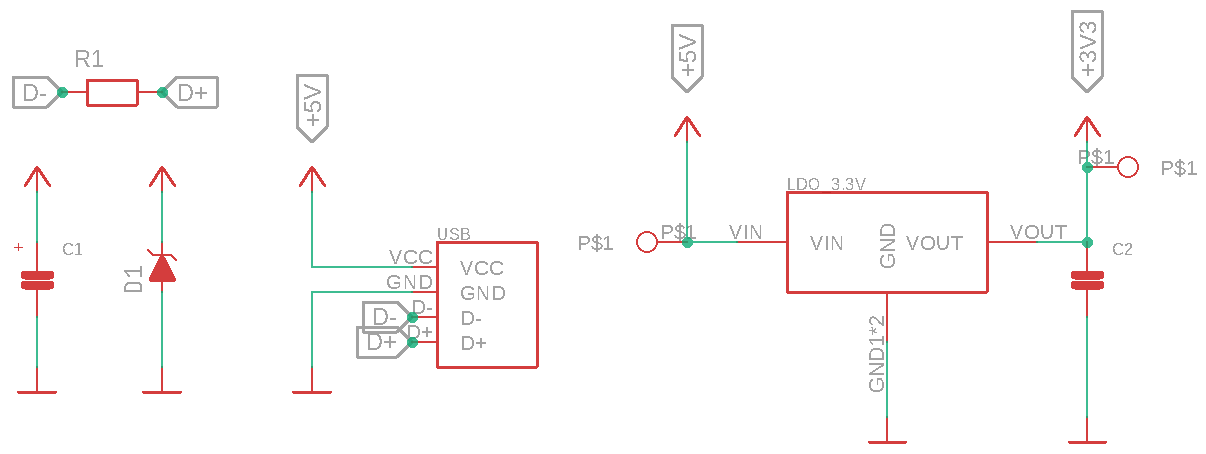
\includegraphics[width=.8\linewidth]{Schaltung-power}	
		\caption{Schaltung Spannungsversorgung}
		\label{fig:Schaltung-power}
	\end{center}
\end{figure}
Abbildung \ref{fig:Schaltung-power} zeigt die Schaltung der Spannungsversorgung des Gerätes. Der Widerstand $R1$ sorgt dafür, dass das Gerät , wie bereits erwähnt, als DCP erkannt wird. Der Elektrolyt-Kondensator $C1$ fungiert als kleiner Puffer, falls die Schaltung für einen kurzen Moment mehr Strom benötigt als die USB-Schnittstelle liefern kann. Der damit einhergehende Spannungsabfall wird zudem kurzzeitig ausgeglichen. Um eventuell zurückfließenden Strom in den USB-Host zu verhindern wird die Diode $D1$ parallel zum 5\,V Potential (VCC) und Ground (GND) geschaltet. Auf der rechten Seite in der Abbildung \ref{fig:Schaltung-power} befindet sich ein LDO-Spannungsregler. Er transformiert die eingehenden 5\,V vom USB-Host auf 3,3\,V herunter und stabilisiert diese gleichzeitig. Laut Tabelle \ref{tab:VDD+IDD} wird ein Strom von maximal ca. 240\,mA aus dem Spannungsregler benötigt. Laut Datenblatt fällt an ihm bei 25\,$^{\circ}$C Umgebungstemperatur und einem Strom von 250\,mA eine Spannung von ca. 100\,mV ab. Der MCU und der SD-Kartensteckplatz können somit mit ausreichend Spannung versorgt werden. Alle anderen Komponenten werden direkt mit den 5\,V der USB-Schnittstelle versorgt, um den LDO-Spannungsregler so wenig wie möglich zu belasten.
% !TEX root = BA-Bauer.tex

\subsection{Autodesk EAGLE}
Die Schaltpläne und das Design der Platine wird in der \textit{Electronic Design Automation} (EDA) Software \textit{EAGLE} der Firma \textit{Autodesk} entwickelt. Innerhalb der Software können Schaltpläne erstellt werden. Anhand dieser Schaltung kann dann ein entsprechendes Layout der zu fertigenden Platine erstellt werden. Zuletzt können Produktionsdaten exportiert werden, mit denen die Platine industriell hergestellt werden kann \cite{eagle_homepage}.\\
Für die Erstellung des Schaltplans und Platinenlayouts wird eine Bauteilbibliothek benötigt. \textit{EAGLE} beinhaltet bereits initial eine große Bibliothek mit verschiedensten Bauteilen vieler Hersteller, jedoch umfasst diese nicht alle am Markt verfügbaren Bauteile. Viele der in dieser Arbeit verwendeten Bauteile befinden sich nicht darin, weswegen eine eigene Bauteilbibliothek erstellt und explizit für die Entwicklung verwendet wird. Zudem soll dadurch das Fehlerrisiko in Bezug auf die Bauteilabmessungen und Pinbelegung reduziert werden. Ein Bauteil der Bauteilbibliothek besteht aus Sicht der Software aus drei Teilen. Dem $symbol$ (Abbildung \ref{fig:eagle-sym}), dem $footprint$ (Abbildung \ref{fig:eagle-foot}) und einem 3D-Modell (Abbildung \ref{fig:eagle-3d}).
\begin{figure}[h]
	\centering
	\begin{minipage}{.3\linewidth}
		\centering
		\includegraphics[height=.1\textheight]{lib-symbol}
		\caption{EAGLE Symbol}
		\label{fig:eagle-sym}
	\end{minipage}
	\hfill
	\begin{minipage}{.3\linewidth}
		\centering
		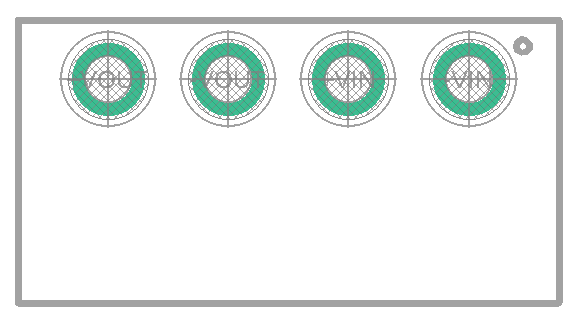
\includegraphics[height=.1\textheight]{lib-footprint}
		\caption{EAGLE Footprint}
		\label{fig:eagle-foot}
	\end{minipage}
	\hfill
	\begin{minipage}{.3\linewidth}
		\centering
		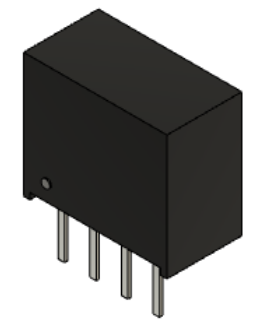
\includegraphics[height=.1\textheight]{lib-3d}
		\caption{EAGLE 3D-Modell}
		\label{fig:eagle-3d}
	\end{minipage}
\end{figure}
Das Symbol wird für die Entwicklung des Schaltplans verwendet und besitzt keine elektrischen Eigenschaften oder Dimensionen. Eine Simulation der Schaltung ist dementsprechend in $EAGLE$ nicht möglich. Die Anschlüsse der Symbole können im Schaltplan mit Leitungen verbunden werden. Um den Schaltplan auf die Hardwareebene zu projizieren, wird ein zugehöriger \textit{footprint} benötigt. Dieser enthält die Dimensionen und Anordnung der entsprechenden Lötstellen des Bauteils, welche in der Regel vom Hersteller des Bauteils zur Verfügung gestellt werden. Im Bibliotheks-Manager in \textit{EAGLE} werden dann die Anschlüsse des Symbols den entsprechenden Lötstellen des \textit{footprints} zugeordnet. Die Verbindung zwischen Schaltplan und Platine ist nun hergestellt. Um  einen noch realistischeren Entwurf der Platine einsehen zu können, kann ein 3D-Modell des Bauteils eingefügt werden. Standard Bauteile wie SMD-Kondensatoren, -Widerstände oder gängige Chip-Gehäuse können mit einem in \textit{EAGLE} integrierten Generator erzeugt werden. Mit den vom Hersteller des Bauteils angegebenen Dimensionen und Toleranzen erzeugt der Generator einen \textit{footprint} mit einem dazugehörigen 3D-Modell des Bauteils. Handelt es sich bei dem Bauteil nicht um ein Standard-Bauteil, so muss der \textit{footprint} in $EAGLE$ und das 3D-Modell in einer externen CAD-Software konstruiert werden. Über den Bibliotheks-Manager kann dann das 3D-Modell bezogen auf den \textit{footprint} dreidimensional platziert werden. Mithilfe der 3D-Modelle kann EAGLE in Verbindung mit der Software \textit{Fusion 360} der Firma \textit{Autodesk} ein 3D-Modell der gesamten Platine inklusive aller Bauteile, für die entsprechende 3D-Modelle in der Bauteilbibliothek existieren, exportieren. Dieses kann dazu verwendet werden, Kollisionen zwischen verschiedenen Bauteilen oder zwischen Bauteilen und Gehäuse vor der Fertigung der Platine zu erkennen oder ein passendes Gehäuse für die Platine zu entwerfen.\\
Mithilfe der in \textit{EAGLE} integrierten sogenannten \textit{Forward-Back-Annotation} werden Änderungen im Schaltplan unmittelbar in das Platinenlayout übertragen. Wird Beispielsweise nur der Wert eines Widerstandes im Schaltplan geändert, so ändert sich auch die Beschriftung des Bauteils auf der Platine. Außerdem werden in der Schaltung gesetzte Verbindungen im Platinenlayout dargestellt. Damit wird das Verlegen von Leiterbahnen vereinfacht und kann fehlerfrei durchgeführt werden. Im Schaltplan nicht bestehende Verbindungen können im Platinenlayout nicht hergestellt werden.
\begin{figure}[h]
	\centering	\begin{minipage}{.35\linewidth}
		\centering
		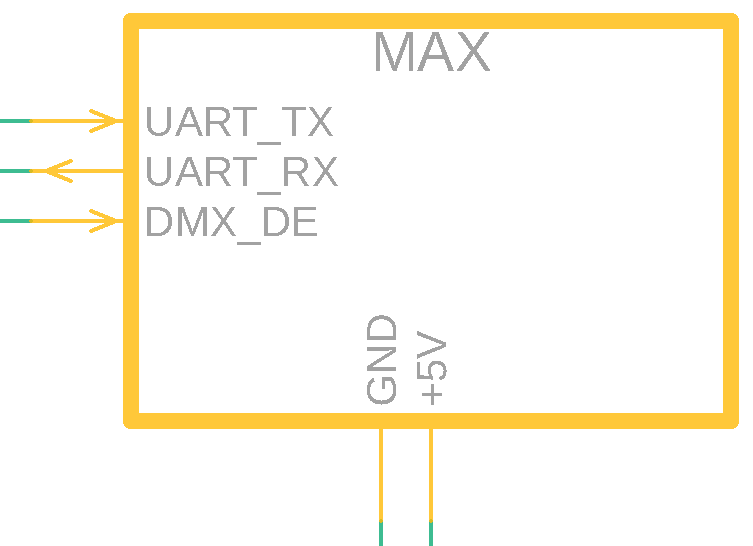
\includegraphics[height=.13\textheight]{Module}
		\caption{Modul $"$MAX$"$}
		\label{fig:module}
	\end{minipage}
	\hfill
	\begin{minipage}{.6\linewidth}
		\centering
		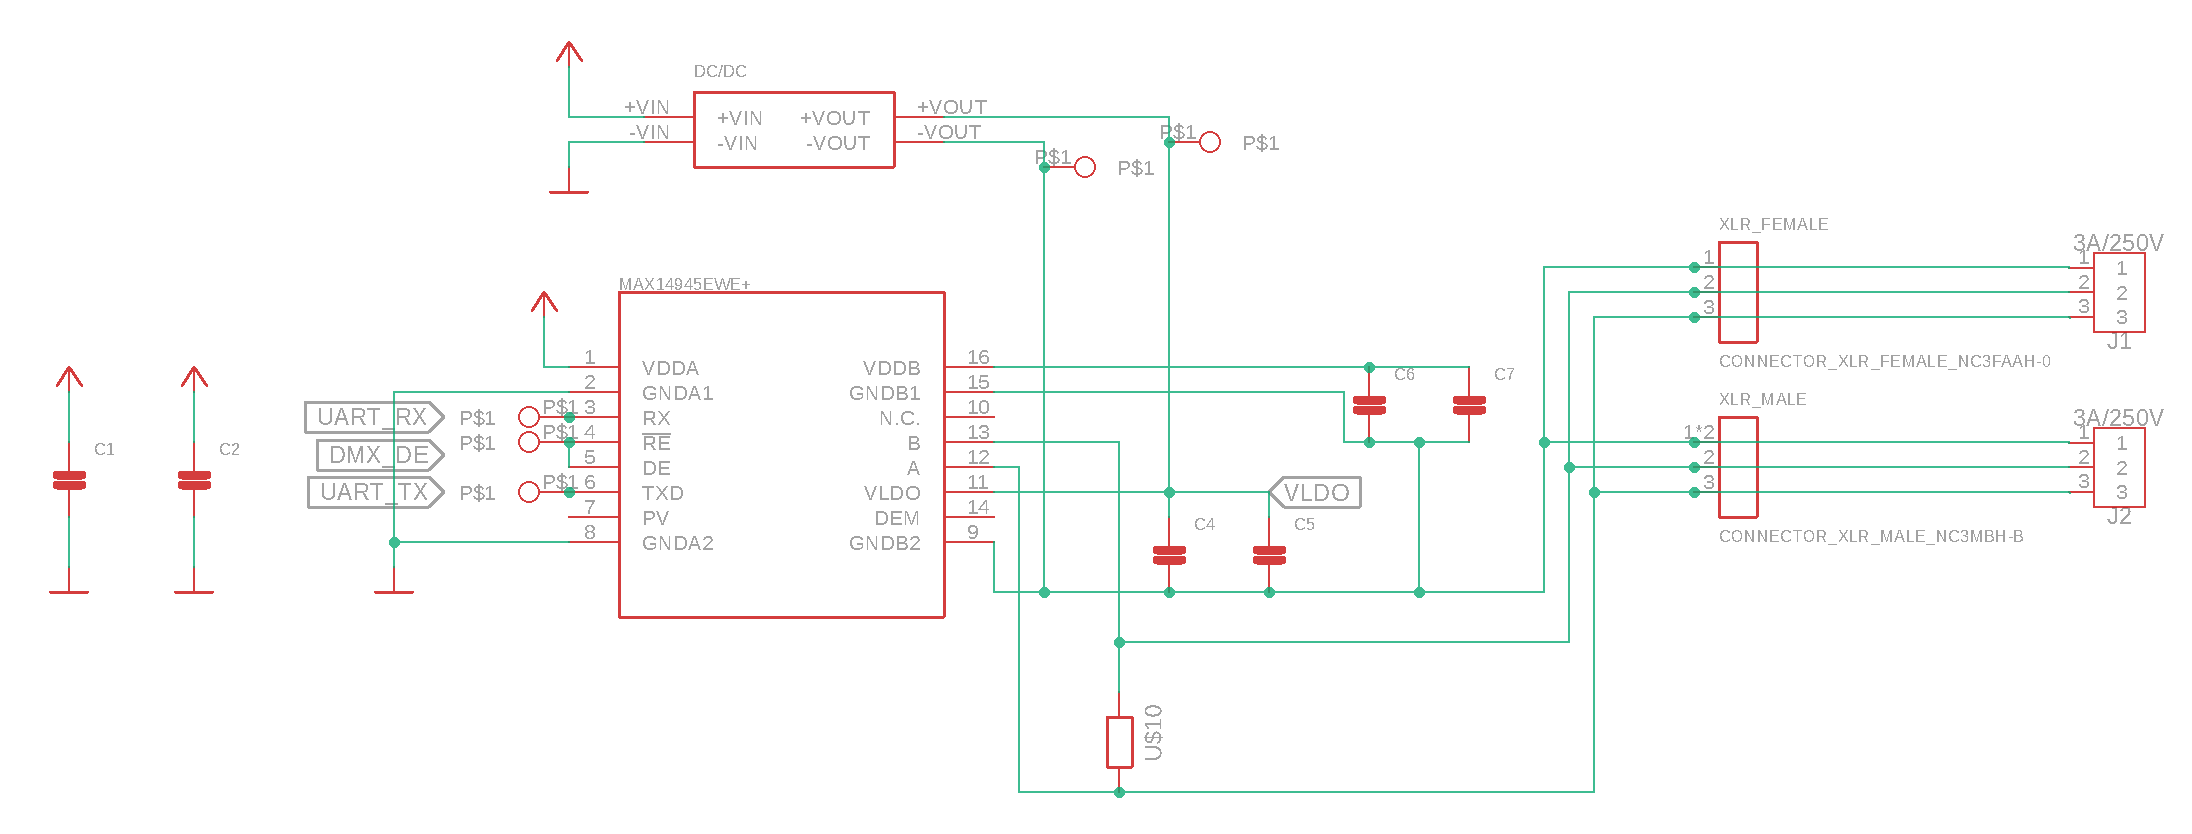
\includegraphics[height=.13\textheight]{Module-schematic}
		\caption{Inhalt des Moduls $"$MAX$"$}
		\label{fig:module-schematic}
	\end{minipage}
\end{figure}
Um die Schaltung möglichst übersichtlich zu gestalten, werden sogenannte \textit{Module} verwendet, durch die komplexe Schaltungen in kleinere \textit{$"$Black-Boxes$"$}\footnote{Box mit Ein-, Ausgängen und unbekanntem Inhalt} heruntergebrochen werden können. Abbildung \ref{fig:module-schematic} und \ref{fig:module} zeigen diese Vereinfachung. Zudem können Module mehrfach in einer Schaltung eingefügt werden. Änderungen in einem Modul wirken sich auf alle eingefügten aus. Verbindungen (grüne Linien in Abbildung \ref{fig:module-schematic}) zwischen Bauteilen werden Namen (\textit{net-names}) zugewiesen, die nur innerhalb des Moduls bekannt sind. Mithilfe der \textit{net-names} können sogenannte \textit{Ports} aus dem Modul herausgeführt werden, womit Verbindungen zu anderen Modulen oder einfachen Bauteilen hergestellt werden können. Pfeile an den $Ports$ signalisieren die Flussrichtung von Signalen, nicht vorhandene Pfeilspitzen signalisieren einen Anschluss einer Spannungsversorgung.\\
% !TEX root = BA-Bauer.tex

\subsection{Platinendesign} \label{sec:PCB-Design}
Das Design der Platine spielt eine wichtige Rolle in der Entwicklung des Gerätes, denn es müssen alle 78\,Komonenten auf ihr Platz finden, sie muss elektrisch und logisch sinnvoll aufgebaut sein und gleichzeitig kompakte Maße haben damit das Endprodukt handlich ist. Zudem kommen einige technische Anforderung von Bauteilen wie die Platzierung der Stützkondensatoren des MCUs, die möglichst nah an ihm platziert werden müssen, hinzu. Außerdem muss der SD-Karten-Steckplatz im nachhinein für den Benutzer zugänglich sein, der Benutzer muss die Taster betätigen, die LEDs leuchten, den LCD sehen können und in der Lage dazu sein die DMX- und das USB-Kabel in die entsprechenden Buchsen zu stecken.
\begin{figure}[h]
	\centering
	\begin{minipage}[t]{0.47\linewidth}
		\centering
		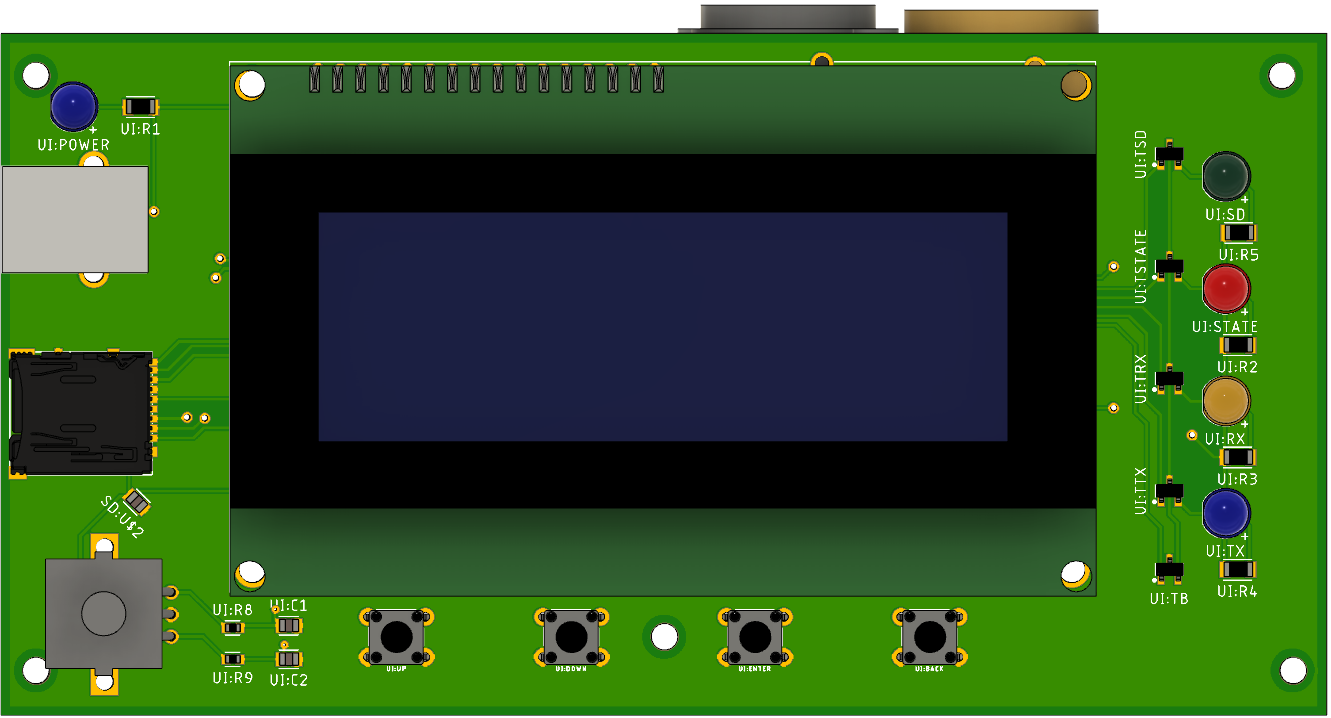
\includegraphics[width=\linewidth]{PCB_top}
		\caption{Platinenvorderseite}
		\label{fig:PCB-top}
	\end{minipage}
	\hfil
	\begin{minipage}[t]{0.47\linewidth}
		\centering
		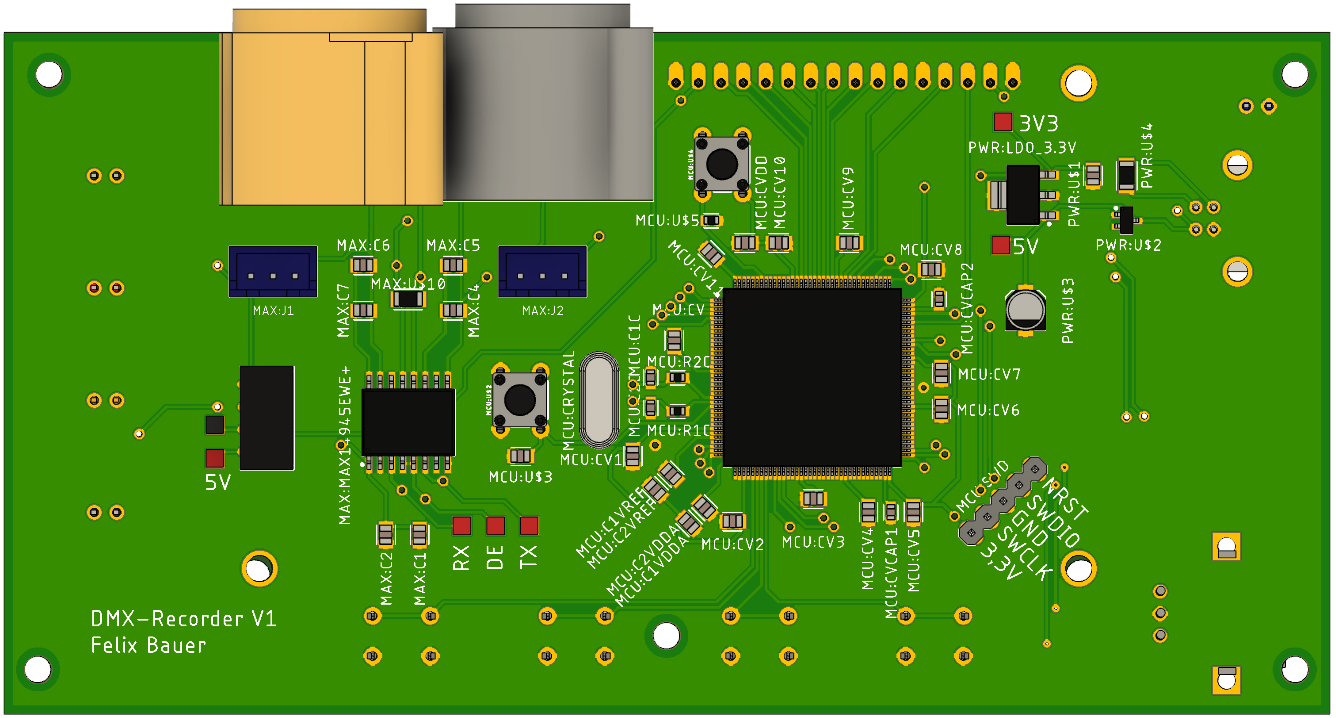
\includegraphics[width=\linewidth]{PCB_bottom}
		\caption{Platinenrückseite}
		\label{fig:PCB-bottom}
	\end{minipage}
\end{figure}\\
Abbildung \ref{fig:PCB-top} und \ref{fig:PCB-bottom} zeigen das Layout der Platine als virtuelles dreidimensionales Modell. 
%Die Platinenentwicklungssoftware \textit{EAGLE}\footnote{https://www.autodesk.de/products/eagle/overview} der Firma \textit{Autodesk} kann in Verbindung mit der ebenfalls von \textit{Autodesk} entwickelten 3D-CAD-Software \textit{Fusion 360}\footnote{https://www.autodesk.de/products/fusion-360/overview} ein virtuelles Modell der Platine automatisiert erstellen. Dieses kann dafür genutzt werden um Kollisionen von einzelnen Komponenten vorab abzuwenden und erleichtert das Konstruieren eines Gehäuses. Zudem gibt es die Möglichkeit die Dimnsionierung der Platine in \textit{Fusion 360} festzulegen und an \textit{EAGLE} zu übergeben. Damit eine möglichst genaue dreidmensionale Abbildung möglich ist, ist es notwendig die einzelnen Komponenten als 3D-Modell zu erstellen. \textit{EAGLE} bietet einen internen Modell-Generator zum generieren von üblichen Komponentenformen. Einige Hersteller bieten außerdem 3D-Modelle als Download an. 
Auf der Platine werden zwei Arten von Komponenten verbaut. Zum einen sogenannte \textit{surface-mount-technology}-Komponenten (SMT-Komponenten), zum anderen \textit{through-hole technology}-Komponenten (THT-Komponenten). SMT-Komponenten werden direkt auf die Oberfläche der Platine gelötet, was keine Notwendigkeit von Löchern in der Platine erfordert. Durch die Oberflächenmotage befindet sich das Bauteil auch auf der selben Seite wie die dazugehörige Lötstelle. Für THT-Komponenten werden Löcher in der Platine benötigt, da die Pins der Komponenten im 90 Grad Winkel zur Oberfläche der Platine gerichtet sind. Diese können unter Umständen nur auf der gegenüberliegenden Seite der Platine verlötet werden. Eine LED zum Beispiel, die bündig mit der Platine verlötet werden soll, kann nur auf der gegenüberliegenden Seite der Platine verlötet werden, da die LED selbst ihre eigenen Pins verdeckt. Damit alle Komponenten frei auf der Platine platziert werden können, wird eine zweiseitige Platine entworfen. Diese besitzt auf der Vorder- und Rückseite eine Kupferschicht, welche mithilfe von sogenannten \textit{Vias}\footnote{Durchkontaktierte Löcher in der Platine} verbunden werden können.
\begin{figure}[h]
	\begin{center}
		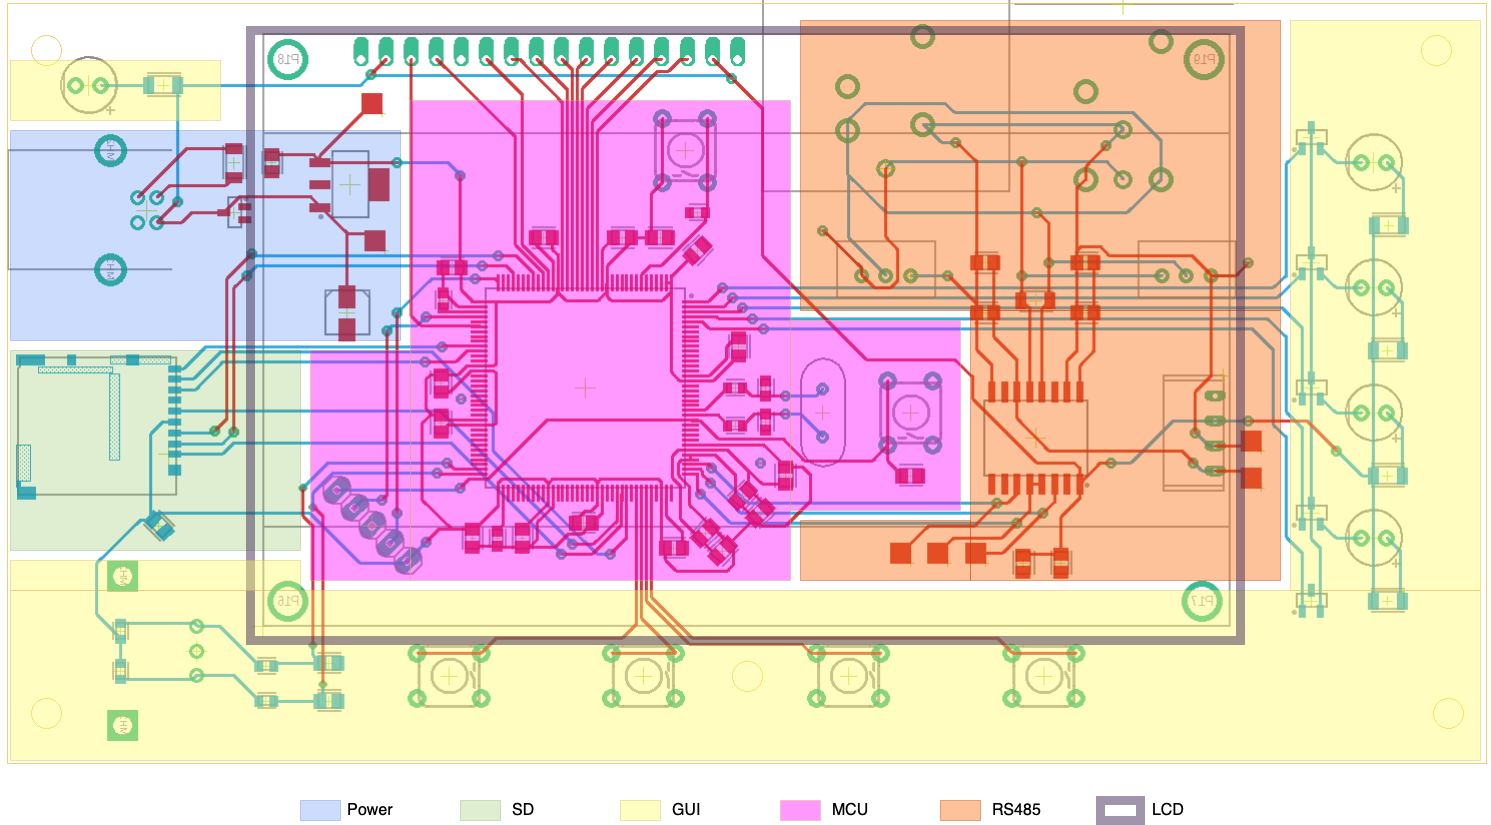
\includegraphics[width=\linewidth]{PCB-Design_mark}
		\caption{Platinenlayout-Aufteilung}
		\label{fig:PCB-Layout}
	\end{center}
\end{figure}
Abbildung \ref{fig:PCB-Layout} zeigt die generelle Aufteilung der Platine. Diese Aufteilung vereinfacht die mögliche Fehlersuche und trägt dazu bei die Leiterbahnlängen zu verkürzen. Alle blau gefärbten $Pads$\footnote{In der Regel rechteckige Lötstellen (freigelegte Kupferflächen) zum verlöten von SMT-Komponenten} und Leiterbahnen befinden sich auf der Vorderseite, alle rot eingefärbten auf der Rückseite der Platine. Die freien Flächen zwischen den Leiterbahnen auf der Ober- und Unterseite sind mit dem 0\,V Potential verbunden. Die grünen Bohrungen sind $Vias$ und durchkontaktiert Bohrungen für die THT-Komponenten.
Der Formfaktor der Platine wird im wesentlichen von dem LCD-Modul vorgegeben, da es bei weitem das größte Bauteil darstellt. Neben dem LCD-Modul muss außerdem Platz für den Encoder, die Taster und LEDs vorhanden und für den Benutzer sichtbar und verwendbar sein. Aus diesem Grund werden das LCD-Modul, die Taster, der Encoder und die LEDs auf der Vorderseite der Platine platziert. Im Zentrum befindet sich das LCD-Modul. Unterhalb des Moduls befinden sich die Taster, rechts davon die LEDs. Die LED, die den Zustand der Spannngsversorgung anzeigt befindet sich oben links um eine Verwechslungen mit der zweiten blauen LED zu verhindern. Der SD-Kartensteckplatz, grün markiert, findet am linken Rand unterhalb der USB-Buchse und Schaltung der Spannungsversorgung, blau markiert, der Platine Platz. Der MCU bildet das Herzstück der Schaltung und befindet sich deswegen  in der Mitte der Platine. Laut Hersteller sollen die Stützkondensatoren möglichst nah am MCU plaziert werden, damit die Induktivität der Leiterbahnen den hohen Stromfluss aus den Kondensatoren heraus nicht beeinträchtigt. \textbf{Erklärung / Quelle} Kritische an den MCU angeschlossene Komponenten sind unter anderem der SD-Kartenslot, der Quartz und der RS485-Treiberchip. Um möglichst wenig Störungen auf die Leiterbahnen einwirken zu lassen sind diese möglichst kurz. Die XLR-Buchsen für die ein- und ausgehenden DMX-Daten befinden sich am oberen Rand der Rückseite der Platine. Sie und die Schaltung des Treiberchips, rot markiert, liegen nah beieinander um auch hier das Störungspotential durch lange Leiterbahnen möglichst gering zu halten.
\input{Hardware/Gehäusedesign}
%Formaterung überprüfen: Einige Bilder stehen nicht am richtigen Platz (durch Seitenumbruch)
	% !TEX root = BA-Bauer

\newpage
\section{Software}
	% !TEX root = BA-Bauer.tex
\newpage
\section{Zusammenfassung}
	% !TEX root = BA-Bauer.tex
\newpage
\section*{Danksagung}
\addcontentsline{toc}{section}{Danksagung}
An dieser Stelle möchte ich allen danken, die mich im Entwicklungsprozess und der Anfertigung dieser Arbeit unterstützt haben.\\
\newline
Zuerst möchte ich mich bei Herrn Prof. Dr. rer. nat. Roman Grothausmann und Herrn Dipl.-Ing. Tobias Bürmann für die Betreuung meiner Bachelorabschlussarbeit bedanken. Durch Ihren Einsatz ist die Bearbeitung dieses Themas erst möglich geworden. Auch die zahlreichen Meetings haben mir wertvolle Anregungen in Bezug auf die Entwicklung gegeben.\\
\newline
Mein Dank gilt außerdem Herrn Stefan Ludwig und das Kollegium des Labors, die mich bei der Herstellung einer Prototyp-Platine unterstützt haben. Sie haben die Platinenfräse der HAWK an die Grenzen des Machbaren gebracht und mich damit in der Entwicklung einen großen Schritt vorangebracht.\\
\newline
Ich danke Jannik Schulz für die wiederkehrende technische Unterstützung im gesamten Entwicklungsprozess.\\
\newline
Ebenfalls bedanke ich mich bei Isabel Klink und Robert Hut, die mich jederzeit tatkräftig mit ihrer Hilfsbereitschaft und Geduld unterstützt und motiviert haben.\\
\newline
Abschließend möchte ich mich bei den Korrekturlesende Isabel Klink, Jannik Schulz, Marcel Trebing und David Wendel bedanken.\\
\newline
Felix Bauer\\
\newline
\newline
\newline
Göttingen, 14.09.2021
	% !TEX root=BA-Bauer.tex

\newpage
\bibliographystyle{unsrt}
\bibliography{Literatur}
	% !TEX root = BA-Bauer.tex

\renewcommand{\listfigurename}{Abbildungen}
\listoffigures
	% !TEX root = BA-Bauer.tex
\newpage
\addcontentsline{toc}{section}{Codeausschnittsverzeichnis}
\renewcommand{\lstlistlistingname}{Codeausschnittsverzeichnis}
\lstlistoflistings
	% !TEX root = BA-Bauer.tex

\newpage
\appendix
\section{Flussdiagramme}
\subsection{Aufnahmefunktion}
\label{fluss:recf}
\begin{figure}[h]
	\begin{center}
		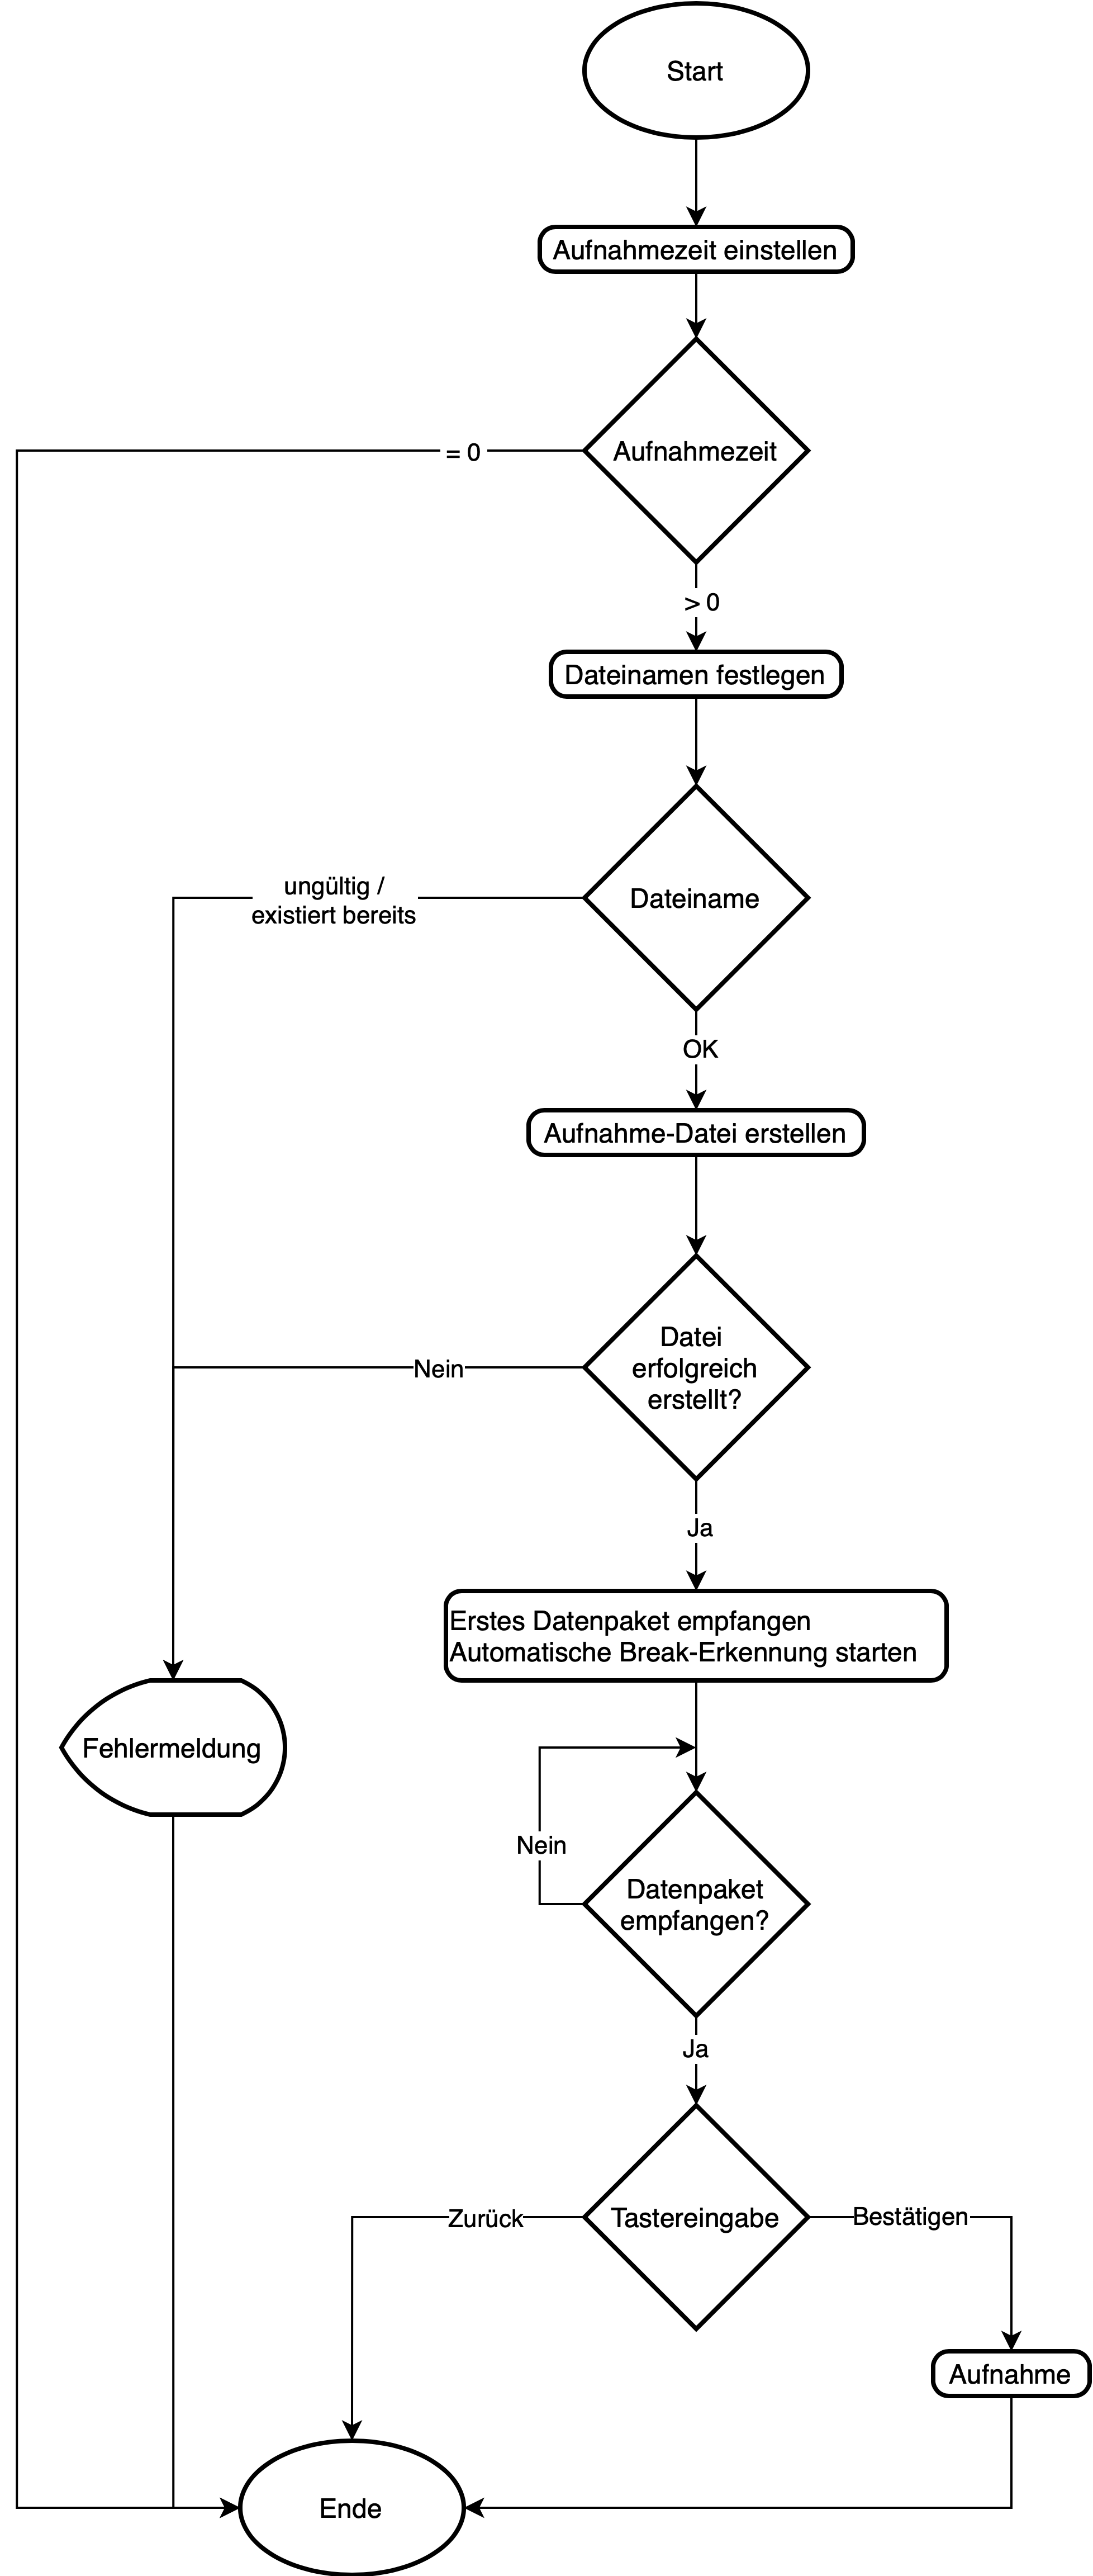
\includegraphics[height=.76\textheight]{Aufnahmefunktion}
	\end{center}
\end{figure}
\newpage
\subsection{Wiedergabefunktion}
\label{fluss:playf}
\begin{figure}[h]
	\begin{center}
		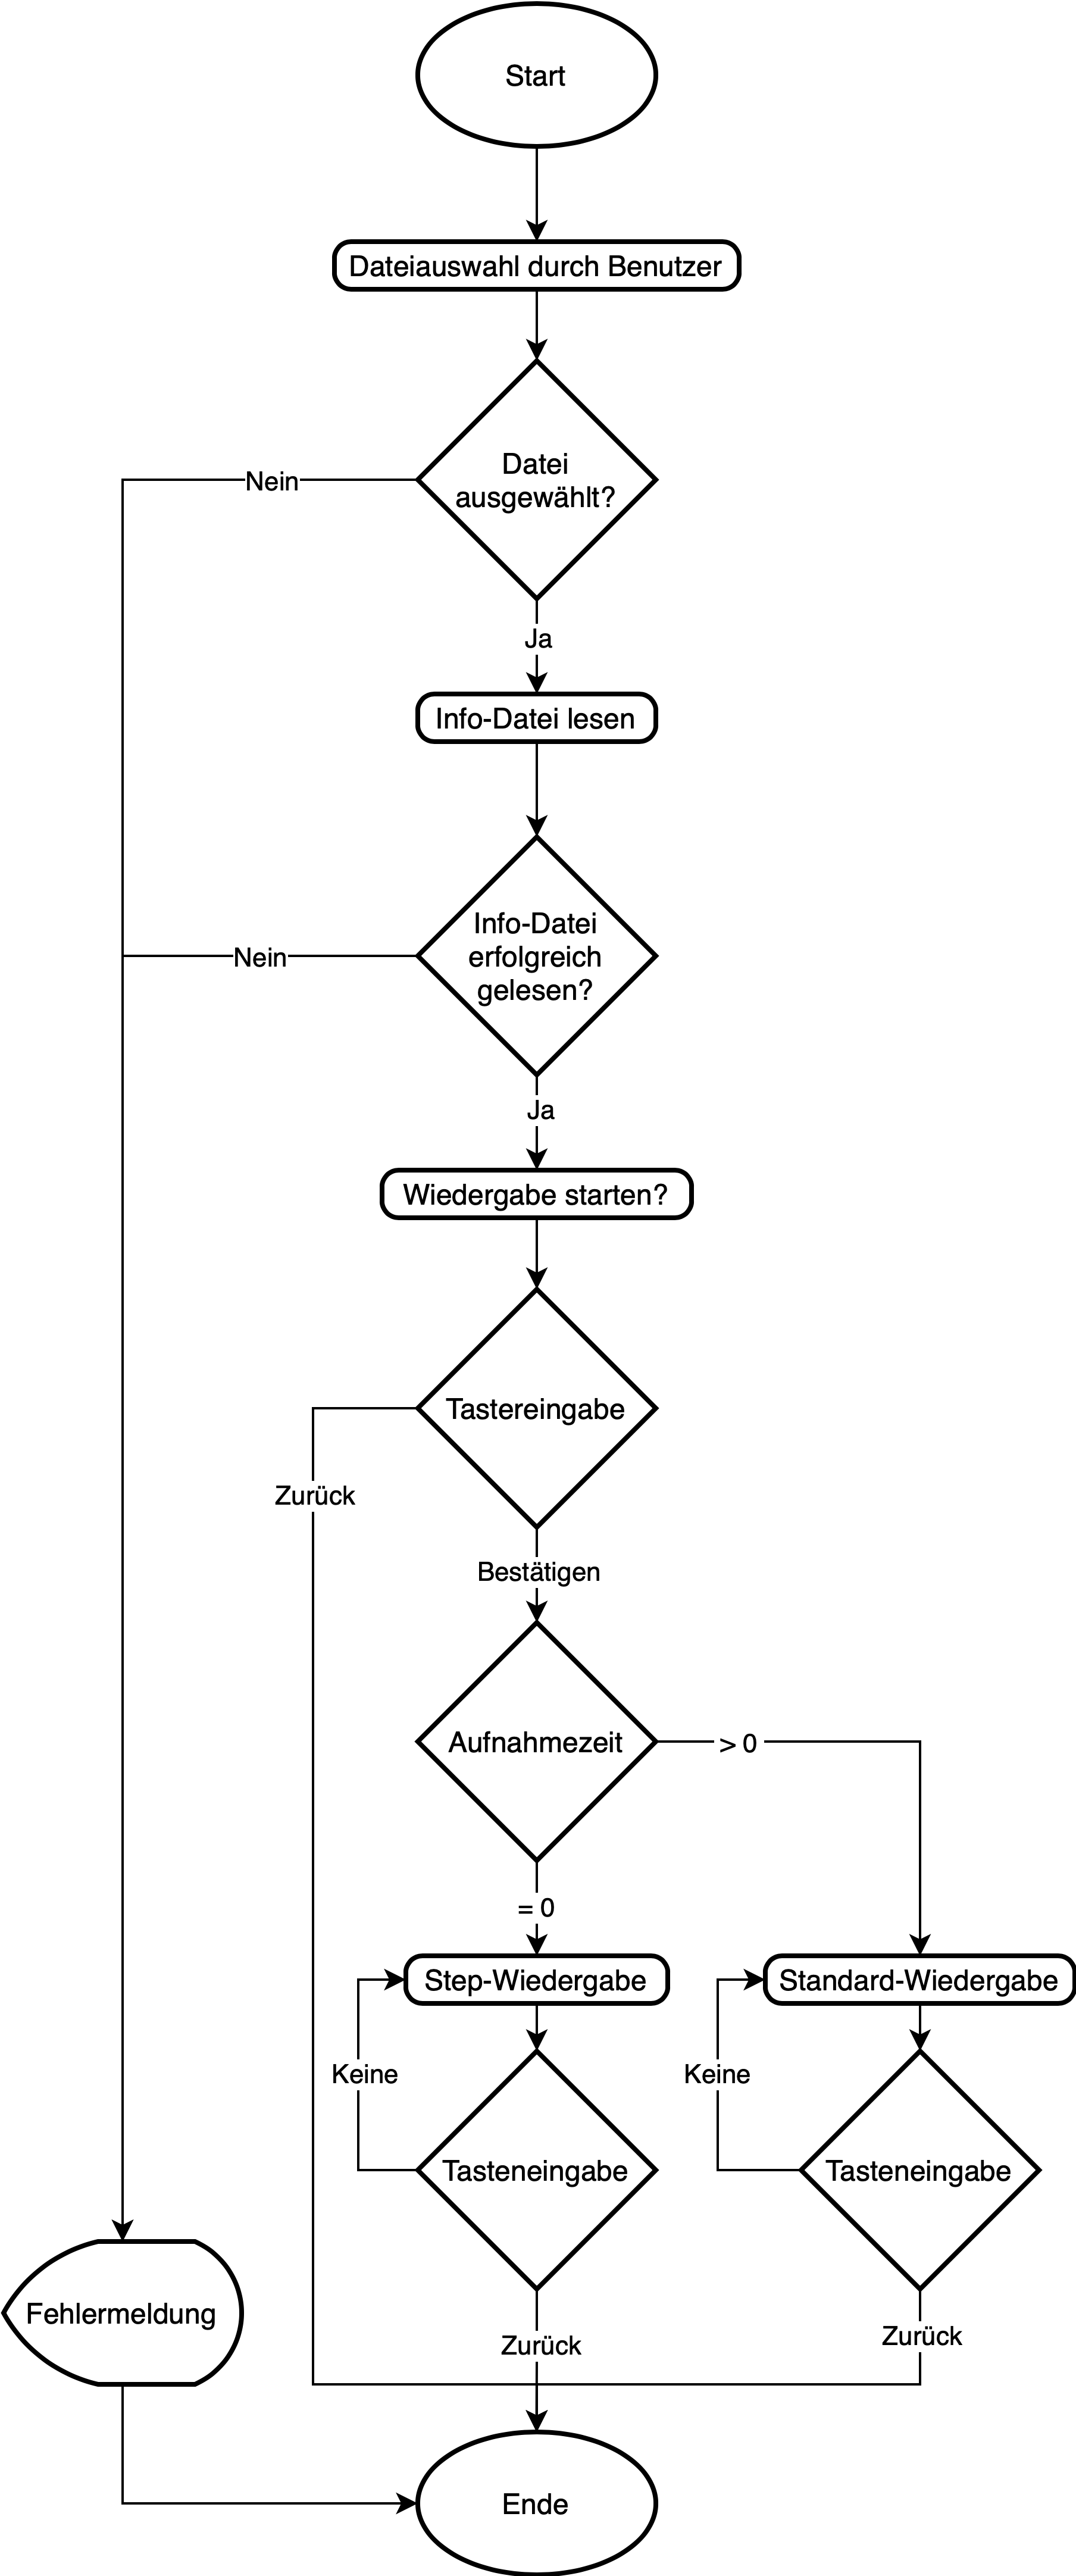
\includegraphics[height=.769\textheight]{Wiedergabefunktion}
	\end{center}
\end{figure}
\newpage
\subsection{Standard Wiedergabe}
\label{fluss:playconti}
\begin{figure}[h]
	\begin{center}
		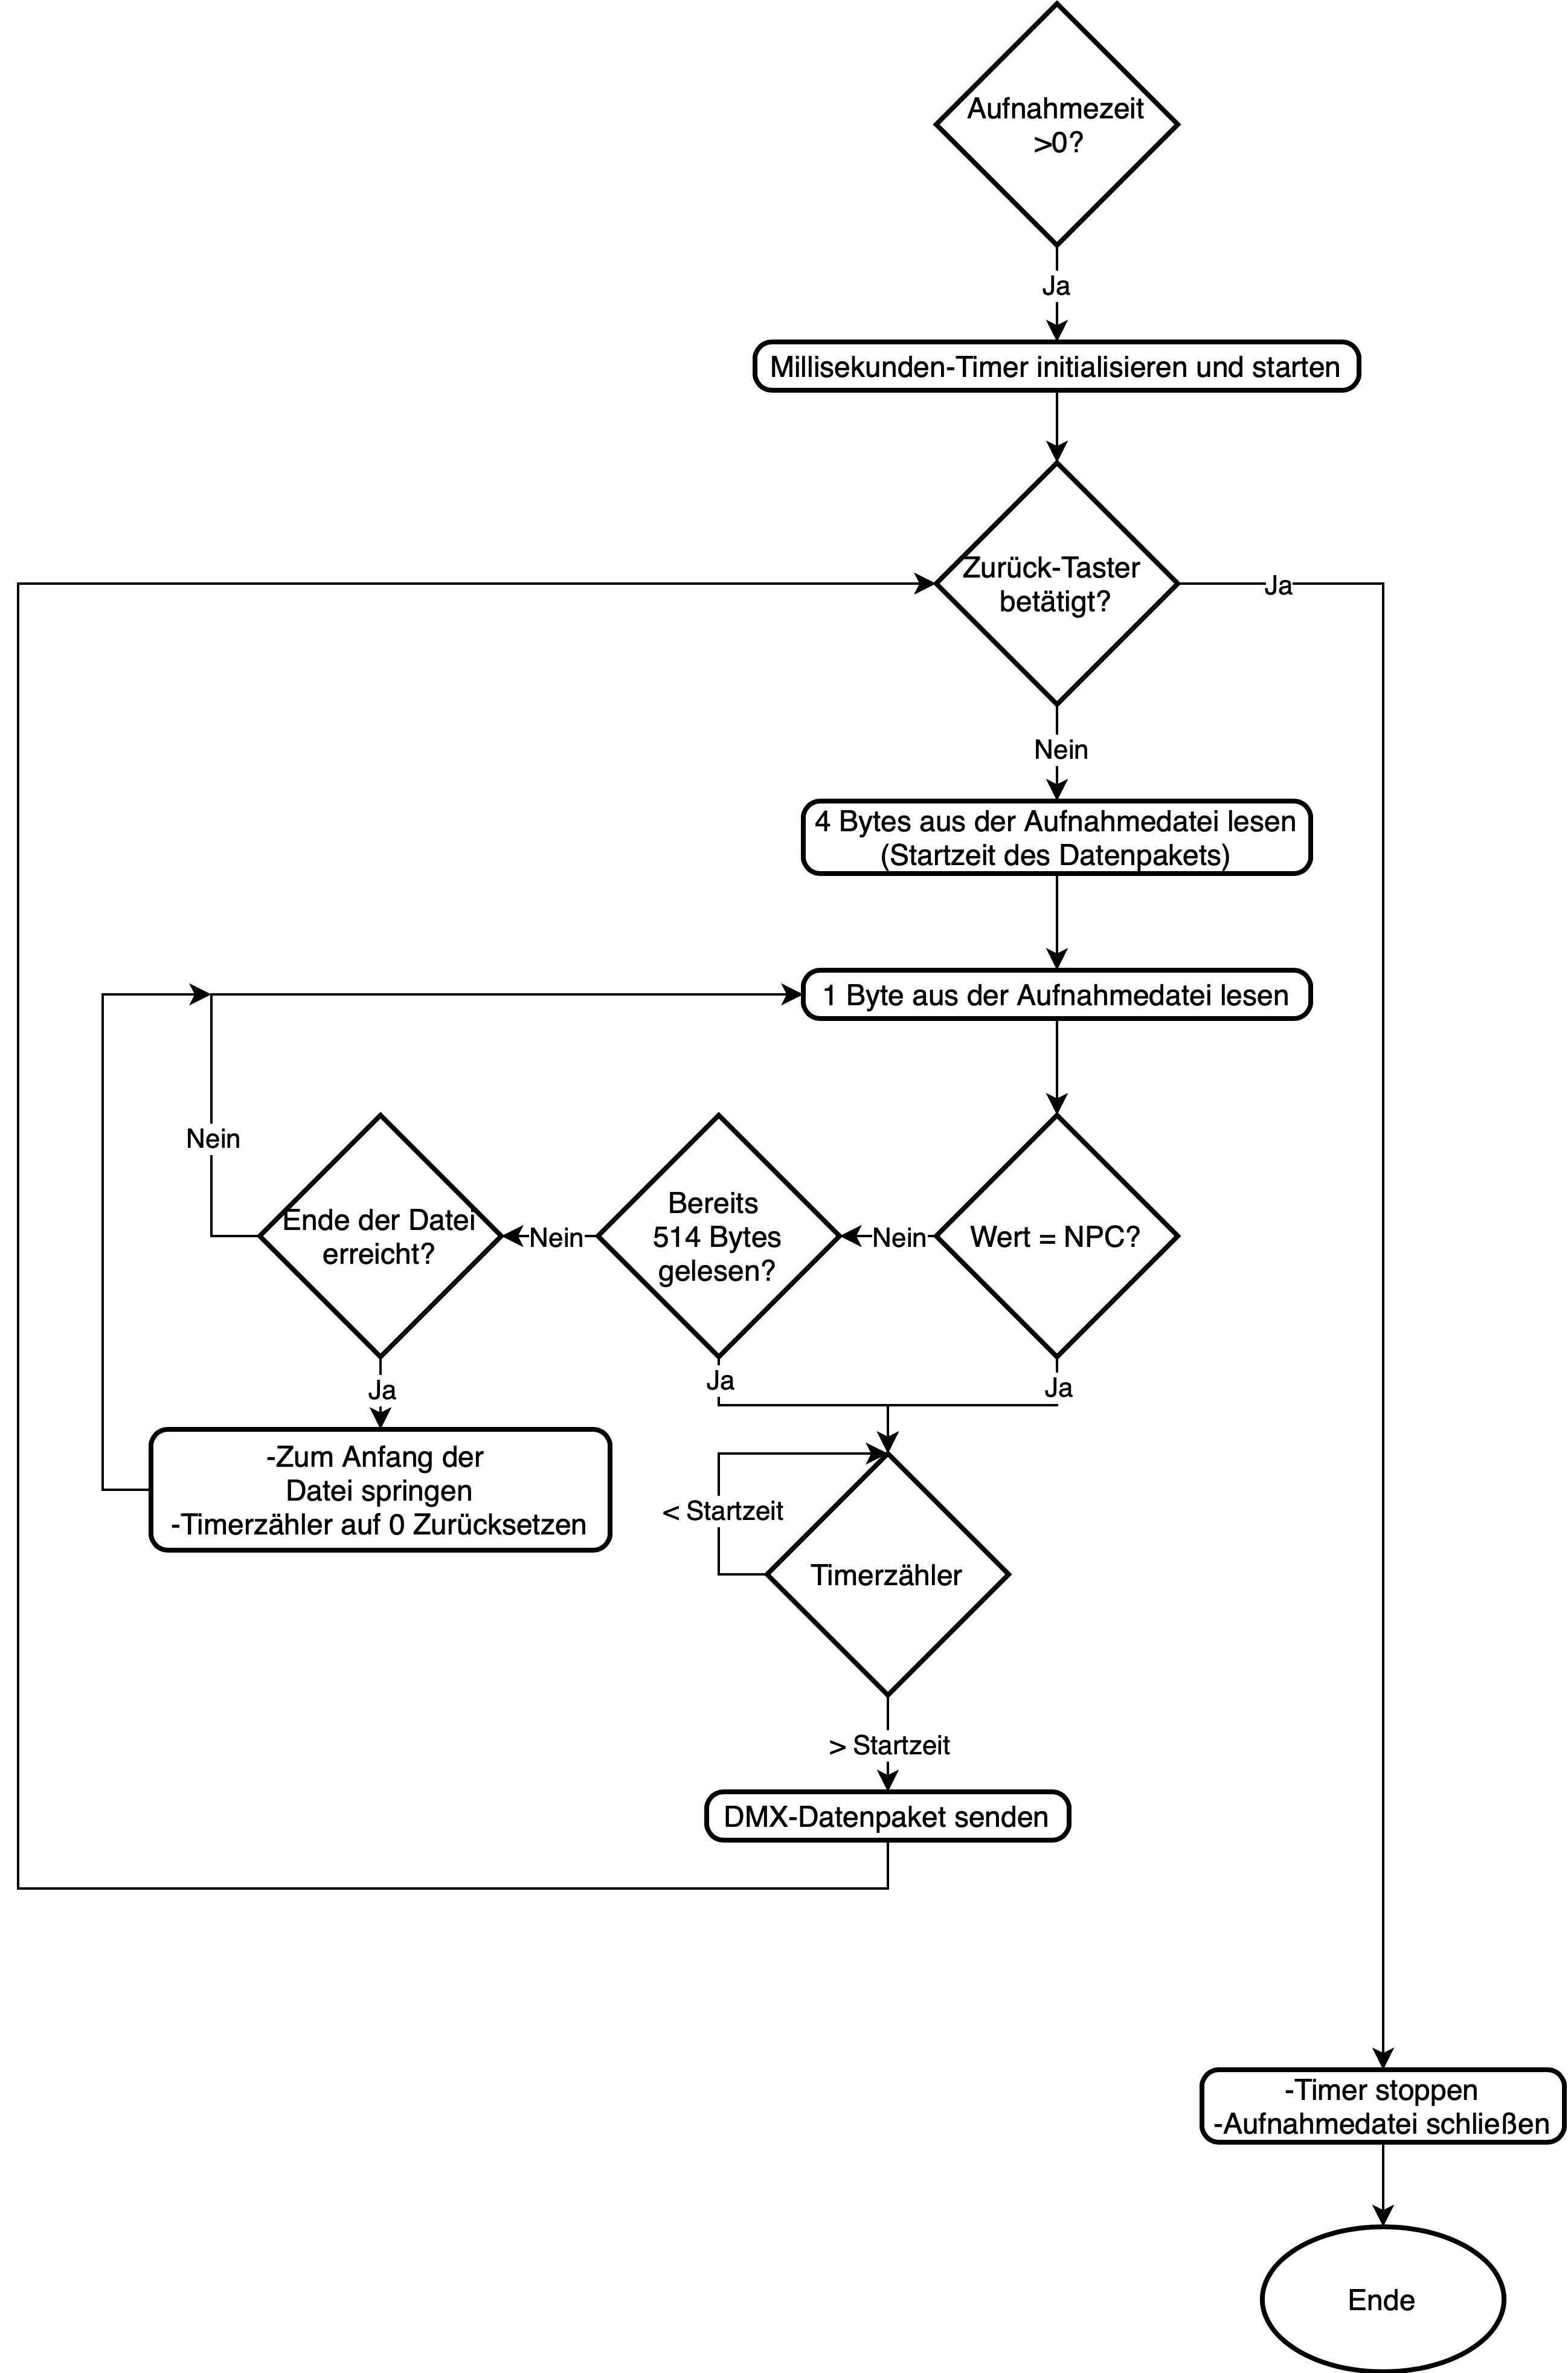
\includegraphics[height=.76\textheight]{Wiedergabe_kontinuierlich}
	\end{center}
\end{figure}
\newpage
\section{Inhalt CD-ROM}
\label{CD-Anhang}
\begin{figure}[h]
	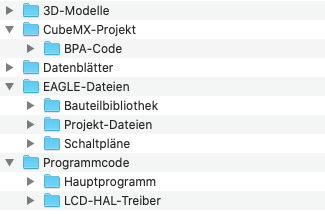
\includegraphics[scale=.7]{CD-Inhalt}
\end{figure}

\end{document}